\documentclass[12pt,a4paper]{report}

\usepackage{dolgozat}
\usepackage{svg}

\begin{document}
\pagestyle{empty} %a címlapon ne legyen semmi=empty, azaz nincs fejléc és lábléc

%A fõiskola logoja
{\large
\begin{center}
\vglue 1truecm
\textbf{\huge\textsc{Szakdolgozat}}\\
\vglue 1truecm

\epsfig{file=cimlap/ME_logo.eps, width=4.8truecm, height=4truecm}\\
\textbf{\textsc{Miskolci Egyetem}}
\end{center}}

\vglue 1.5truecm %függõleges helykihagyás

%A szakdolgozat címe, akár több sorban is
{\LARGE
\begin{center}
\textbf{Hexagonális térképek procedurális generálása}
\end{center}}

\vspace*{2.5truecm}
%A hallgató neve, évfolyam, szak(ok), a konzulens(ek) neve
{\large
\begin{center}
\begin{tabular}{c}
\textbf{Készítette:}\\
Sedlák Bálint\\
Programtervező informatikus
\end{tabular}
\end{center}
\begin{center}
\begin{tabular}{c}
\textbf{Témavezetõ:}\\
Piller Imre
\end{tabular}
\end{center}}
\vfill
%Keltezés: Hely és év
{\large
\begin{center}
\textbf{\textsc{Miskolc, 2017}}
\end{center}}

\newpage


\pagestyle{myheadings}

%Feladatkiiras
\begin{flushleft}
\textsc{\bfseries Miskolci Egyetem}\\
Gépészmérnöki és Informatikai Kar\\
Alkalmazott Matematikai Intézeti Tanszék\hspace*{4cm}\hfil \textbf{Szám:}
\end{flushleft}
\vskip 0.5cm
\begin{center}
\large\textsc{\bfseries Szakdolgozat Feladat}
\end{center}
\vskip 0.5cm
Sedlák Bálint (GMZLQN) programtervező informatikus jelölt részére.\newline

\noindent\textbf{A szakdolgozat tárgyköre:} számítógépi grafika, 3D modellezés, játékfejlesztés\newline

\noindent\textbf{A szakdolgozat címe:} Hexagonális térképek procedurális generálása\newline

\noindent\textbf{A feladat részletezése:}

\vfill

\noindent\textbf{Témavezető:} Piller Imre (egyetemi tanársegéd) \newline

% \noindent\textbf{Konzulens(ek):} (akkor kötelezõ, ha a témavezetõ nem valamelyik matematikai tanszékrõl való; de persze lehet egyébként is)\newline

\noindent\textbf{A feladat kiadásának ideje:}\newline

%\noindent\textbf{A feladat beadásának határideje:}

\vskip 2cm

\hbox to \hsize{\hfil{\hbox to 6cm {\dotfill}\hbox to 1cm{}}}

\hbox to \hsize{\hfil\hbox to 3cm {szakfelelős}\hbox to 2cm{}}

\newpage

\vspace*{1cm}  
\begin{center}
\large\textsc{\bfseries Eredetiségi Nyilatkozat}
\end{center}
\vspace*{2cm}  

Alulírott \hbox to 7cm{\dotfill}; Neptun-kód: \hbox to 3.5cm{\dotfill} a Miskolci Egyetem Gépészmérnöki és Informatikai Karának végzős \hbox to 3.5cm{\dotfill} szakos hallgatója ezennel büntetőjogi és fegyelmi felelősségem tudatában nyilatkozom és aláírásommal igazolom, hogy \hbox to 9.5cm{\dotfill}
című szakdolgozatom/diplomatervem saját, önálló munkám; az abban hivatkozott szakirodalom
felhasználása a forráskezelés szabályai szerint történt.\\

Tudomásul veszem, hogy szakdolgozat esetén plágiumnak számít:
\begin{itemize}
\item szószerinti idézet közlése idézőjel és hivatkozás megjelölése nélkül;
\item tartalmi idézet hivatkozás megjelölése nélkül;
\item más publikált gondolatainak saját gondolatként való feltüntetése.
\end{itemize}

Alulírott kijelentem, hogy a plágium fogalmát megismertem, és tudomásul veszem, hogy
plágium esetén szakdolgozatom visszautasításra kerül.

\vspace*{3cm}

\noindent Miskolc, \hbox to 2cm{\dotfill} .év \hbox to 2cm{\dotfill} .hó \hbox to 2cm{\dotfill} .nap

\vspace*{3cm}

\hspace*{8cm}\begin{tabular}{c}
\hbox to 6cm{\dotfill}\\
Hallgató
\end{tabular}



\newpage

\noindent 1.

\begin{tabular}{cl}
&szükséges (módosítás külön lapon) \\
A szakdolgozat feladat módosítása& \\
& nem szükséges\\
&\\
\hbox to 4cm{\dotfill}&\multicolumn{1}{c}{\hbox to 5cm{\dotfill}}\\
dátum& \multicolumn{1}{c}{témavezető(k)}
\end{tabular}
\vskip1.5mm

\noindent 2. A feladat kidolgozását ellenőriztem:

\vskip1.5mm

\begin{tabular}{l@{\hspace*{4cm}}l}
témavezető (dátum, aláírás):& konzulens (dátum, aláírás):\\
\dotfill&\dotfill\\
\dotfill&\dotfill\\
\dotfill&\dotfill
\end{tabular}

\vskip1.5mm

\noindent 3. A szakdolgozat beadható:

\vskip1.5mm

\begin{tabular}{@{\hspace*{1.3cm}}c@{\hspace*{2.1cm}}c}
\hbox to 4cm{\dotfill}&\multicolumn{1}{c}{\hbox to 5cm{\dotfill}}\\
dátum& \multicolumn{1}{c}{témavezető(k)}
\end{tabular}

\vskip1.5mm

\noindent 4.
\begin{tabular}[t]{@{}l@{\hspace*{1mm}}l@{\hspace*{1mm}}l@{}}
A szakdolgozat& \hbox to 3.5cm{\dotfill} &szövegoldalt\\
              & \hbox to 3.5cm{\dotfill} &program protokollt (listát, felhasználói leírást)\\
              &\hbox to 3.5cm{\dotfill}   &elektronikus adathordozót (részletezve)\\
              &\hbox to 3.5cm{\dotfill} & \\
              &\hbox to 3.5cm{\dotfill} &egyéb mellékletet (részletezve)\\
              &\hbox to 3.5cm{\dotfill} &\\
\end{tabular}
\newline tartalmaz.

\vskip1.5mm

\begin{tabular}{@{\hspace*{1.3cm}}c@{\hspace*{2.1cm}}c}
\hbox to 4cm{\dotfill}&\multicolumn{1}{c}{\hbox to 5cm{\dotfill}}\\
dátum& \multicolumn{1}{c}{témavezető(k)}
\end{tabular}

\noindent 5.

\begin{tabular}{ll}
&bocsátható\\
A szakdolgozat bírálatra& \\
& nem bocsátható\\
\end{tabular}

\vskip1.5mm

\noindent A bíráló neve: \hbox to 8cm{\dotfill}

\vskip4mm

\begin{tabular}{@{\hspace*{1.3cm}}c@{\hspace*{2.1cm}}c}
\hbox to 4cm{\dotfill}&\multicolumn{1}{c}{\hbox to 5cm{\dotfill}}\\
dátum& \multicolumn{1}{c}{szakfelelős}
\end{tabular}

\noindent 6.
\begin{tabular}[t]{@{}l@{\hspace*{1mm}}l@{\hspace*{1mm}}l@{}}
A szakdolgozat osztályzata& &\\
&a témavezető javaslata:& \hbox to 3cm{\dotfill}\\
&a bíráló javaslata:& \hbox to 3cm{\dotfill}\\
&a szakdolgozat végleges eredménye:& \hbox to 3cm{\dotfill}
\end{tabular}

\vspace*{4mm}

\noindent Miskolc, \hbox to 4.5cm{\dotfill} \hspace*{2.5cm}
\begin{tabular}[t]{cc}
\hbox to 6cm{\dotfill}\\
a Záróvizsga Bizottság Elnöke
\end{tabular}


\tableofcontents

\newpage

\pagestyle{fancy}

\Chapter{Bevezetés}

A szakdolgozatom célja egy olyan procedurális generálási mód kidolgozása, amellyel izometrikus grafikájú játékokhoz változatos térképeket lehet előállítani. A térképek hexagon alapúak. A dolgozat azt a többlépcsős folyamatot mutatja be, amely során a program a nagyobb összefüggő egységek meghatározása után sorban határozza meg a különböző részletességi szinteken lévő elemeket.

A szoftver C\# programozási nyelven készül. A C\# ismerete és a fejlesztéshez való alkalmazhatósága miatt esett a választásom erre a nyelvre, ezáltal a fejlesztéshez használt játékmotornak a Unity-t, fejlesztő környezetnek pedig a Visual Studio-t választottam Windows 10 platformon.


\chapter{Procedurális generálás}

\section{Procedurális generálás áttekintése}

\noindent A procedurális generálás egy módszer arra, hogy tartalmat hozzunk létre egy algoritmus segítségével. Tehát ebben az esetben a programozó nem “saját maga” fog előállítani tartalmat (esetünkben például egy térképet vagy egyéb objektumokat), hanem ő csak egy algoritmust fog készíteni ami helyette állítja elő a tartalmat. A számítógépi grafikában gyakran használják a véletlenszerű generálás fogalmat erre a jelenségre, amivel gyakran állítanak elő textúrákat vagy modelleket a játékokhoz. A procedurális generálás egyik nagy előnye az,  hogy nagy mennyiségű tartalom készíthető a játékhoz úgy, hogy emellett ez a tartalom még kevesebb helyet is foglaljon. Mindazonáltal, ha sikerül ezt a technikát jól alkalmaznunk, akkor a generálásnak a véletlenszerűségét kihasználva változatosabb, kevésbé előre megjósolható pályákat vagy feladatokat készíthetünk, ezáltal növelve a játékélményt.  

\section{Előfordulása a játékokban}

\noindent A műfaj egyik már-már legendásnak számító alkotása a \textit{Bethesda Softworks} által 1996-ban kiadott \textit{The Elder Scrolls II: Daggerfall}, amely egy nyílt világú szerepjáték. A játékban a játékosnak lehetősége van például létrehozni saját varázslatokat különböző hatásokkal, amiknek a költségét az algoritmus fogja meghatározni azáltal, hogy milyen erősségűre sikerült a varázslat. Hasonló módszerrel oldották meg a játékban a felszerelés fejlesztési rendszert, a ház és hajó vásárlást, a ruhák és felszerelések változatosságát. A játék ezenfelül rendelkezett dinamikus politikai rendszerrel. A politikai rendszerben számított az,  hogy a karakter milyen céhnek volt a tagja, milyen vallású volt, milyen feladatokat és küldetéseket, cselekedeteket hajtott végre. Ez alapján a politikai rendszer alapján dőlt el, hogy a különböző NPC-k (számítógép által irányított karakterek) hogyan viszonyultak a játékoshoz. 
\newline
\newline A \textit{Bethesda} állítása alapján a játék térképének a mérete közel azonos a Brit-szigetek méretével, számszerűen 229 848 $km^2$. A játékban több mint 15 000 település és város kapott helyett. Emellett több mint 750 000 NPC is szerepel. 
\newline
\newline A \textit{The Elder Scrolls II: Daggerfall}-nak az egyik legnagyobb negatívuma a generáláshoz felhasznált limitált mennyiségű építőelem volt, amiből a városok és a falvak épületei épültek fel. Ez sok játékosnál monotónia érzetet keltett. 
\newline
\newline 2002-ben a sorozat következő részében az alkotók már tanultak korábbi hibáikból és a \textit{The Elder Scrolls III: Morrowind} esetében a korábbinál jóval kisebb térképet készítettek ami körülbelül $0,01 \%$-a volt az előzőnek, számokban kifejezve 24 $km^2$. Viszont a kisebb térképnek köszönhetően a világot sokkal részletgazdagabbá tudták tenni. A városok, települések, és az NPC-k is sokkal egyedibb megjelenést kaptak.
\newline
\newline Az alkalmazáshoz amit készítettem megjelenésre leginkább a \textit{Civilization} széria hasonlít, amely az első négy részében még négyzetrácsot alkalmazott a térkép ábrázolásához, de 2010-ben a \textit{Civilization V} -ben már áttértek a hexagon alapú térképre. Általánosságban elmondható a \textit{Civilization} sorozat játékairól, hogy a térképek procedurálisan generáltak már 1990 óta, kivéve a Föld térképet (bár ebben is előfordulhattak kisebb eltérések játékról-játékra). A \textit{Civilization V} esetén a véletlenszerű térképek miatt majdnem minden esetben procedurálisan kellett generálni a hegyeket, folyókat, városokat, utakat. A játékos a játék kezdete előtt meghatározhatja, hogy milyen alakú legyen a térkép és annak egyéb tulajdonságait a széleskörű beállítási lehetőségek által. A játékosnak módjában áll létrehozni kis szigetekből álló szigetcsoportot (Archipeligo) egy nagyobb kontinenst (Pangaea) vagy akár olyan térképet ami két nagyobb kontinensből áll (Continents). A \textit{Civilization} procedurális generátorától a legtöbb esetben azt kapjuk amit várunk tőle, már előre tudható, hogy milyen térképet fog generálni. Semmi váratlan vagy szokatlan. De a \textit{Civilization} esetében pontosan erre is van szükségünk.
\newline
\newline Manapság talán a legismertebb játék ami procedurális generálást alkalmaz az a \textit{Minecraft}. A \textit{Minecraft} az egész játékvilág létrehozására algoritmusokat használ, ami óriási átalakításokon ment át az évek során. A játékmenet alapvetően két fő elemre építkezik a felfedezésre és az építésre. A felfedezés során lehet hozzájutni különböző nyersanyagokhoz amikből aztán később lehet építkezni. A \textit{Minecraft}-ban a felfedezést az teszi izgalmassá, hogy már-már végtelennek számító véletlenszerűen generált térképet sikerült megtölteni szokatlan természeti jelenségekkel amelyek néhány esetben a valóságon alapulnak de sok más esetben a fikcióval keveredik. Könnyen belátható, hogy egy jól működő procedurális generálás nélkül a \textit{Minecraft} nem lenne olyan sikeres. Az elméletileg végtelen térkép, a változatos növényzet és a kifejezetten jónak számító procedurális generáló algoritmus ellenére is azzal kell szembesülnünk, hogy rengeteg ismétlődéssel találkozunk. Globális szinten, ha jobban megfigyeljük a környezetet feltűnhet hogy 10-ből 9-szer nagyon hasonló képet látunk. Az apró részletek különbözőek lesznek de egészét tekintve nagyon sok hasonlóságot tudunk felfedezni a különböző részek között, a tipikus füves területek mellett pár kockányira mindig feltűnik egy-egy hegy, mivel így épülnek fel a különböző területek az algoritmusban. 
\newline
\newline \textit{A No Man’s Sky} bejelentésekor hatalmas vihart kavart, hiszen olyan egyedülálló játékélményt ígért, amit még más játékban nem tapasztalhattunk. Gyakorlatilag végtelen méretű univerzumot ígért, ahol minden bolygó és minden lény procedurálisan generált. A végeredmény csalódást keltő volt, hiszen a vártakkal ellentétben mégsem volt minden egyedi és a megvalósítással is akadtak problémák. Főleg a bolygók esetében volt megfigyelhető, hogy a különböző nyersanyagokat leszámítva nem volt túl sok különbség. A játéknak a procedurális generátora túlságosan véletlenszerűen generált bizonyos lényeket, ezáltal furcsa és nem túl realisztikus megjelenést kölcsönözve nekik. A játék generáló algoritmusa nem volt eléggé kidolgozott, ahhoz, hogy valóra váltsa az ígérteket.
\newline
\newline A \textit{Spore}-ban a fő hangsúly a különböző lények és bolygók generálásán volt. A játékban szereplő összes lény teljes mértékben generált volt és semmilyen modellt nem használtak a létrehozásukhoz. Ezért az összes élőlény animációja akkor jött létre, amikor a játékos megalkotta őket, az alapján ahogyan megalkotta őket. Például, ha a játékos egy négy lábú lényt készített, akkor arra számíthatott, hogy úgy fog mozogni mint egy ló. A játék legelső bemutatásakor a készítők egy három lábú lényen mutatták be, hogy hogyan működik a folyamat és az algoritmus megállapította, hogy hogyan fog mozogni az általuk létrehozott lény. A játék különböző szakaszaiban a lények különböző képességekre tesznek szert vadászat, evés, úszás, különböző objektum megfogása, tánc amiket szintén algoritmus generál. A készítők bemutattak különböző előre elkészített lényeket, amelyek realisztikusan mozogtak annak ellenére, hogy például volt olyan amelyiknek több feje és 6 lába volt.
\newline
\newline Az ismertetett példák többségében megfelelően használták a procedurális generálást a tartalom előállítására. A \textit{Civilization} arra használta, hogy elrendezze a terepet és a nyersanyagokat a térképen. A \textit{Minecraft} sikerének az egyik oka a procedurálisan generált térkép. Azt láthatjuk, hogy magával a procedurális generálásnak a használatával semmi probléma nincs, abban az esetben, ha megfelelően alkalmazzák azt. Megfelelő alatt azt értem, hogy amikor valami különös, egyedi megjelenés a cél vagy a játék szempontjából szükségét látják annak, hogy a játékos minden alkalommal más lényekkel vagy térképpel találkozzon, ilyen esetekben hozzá tud adni a játékhoz. De amikor túlzásba viszik vagy nincs megfelelően kidolgozva, akkor könnyen tönkreteheti vagy elvehet a játékélményből. 
\newline
\newline Első ránézésre úgy tűnhet, mintha a procedurális generálás valami varázslat lenne a játékfejlesztésben, ami egy csapásra megold minden problémát. Mivel elméleti síkon végtelen számú variációjú tartalmat képes generálni, ami végtelen számú újrajátszhatósági értéket jelentene a játék számára, mivel minden egyes alkalommal mást kellene látnunk.
\newline
\newline Gyakorlatban ez nem így működik, gyakran pont az ellenkezőjét sikerül elérni és nagyon nehéz megtalálni a helyes egyensúlyt. Ezáltal beláthatjuk, hogy a kevesebb néha több, hogy klasszikust idézzek.


\Chapter{Rácsok összehasonlítása}

Legyen szó társasjátékról vagy számítógépes játékról, az egyik leggyakrabban használt rács a négyzetrács. Egyszerû, könnyen kezelhetõ és jól illeszthetõ a számítógép kijelzõjére. A cellák pozícióit a Descartes-féle derékszögû koordináta-rendszer (x, y) segítségével határozhatjuk meg. Kirajzolásához ismernünk kell a cellai méreteit (szélesség, magasság) illetve a rács méreteit (oszlopok, sorok száma). A nyilvántartáshoz ismernünk kell a viszonyítási pontot (origó), illetve tudnunk kell az objektum pozicióját (x, y).

Könnyen kezelhetõsége mellett viszont van egy nagy hátránya:
Egy négyzetnek nyolc szomszédja van. Oldalain keresztül vízszintesen, valamint függõlegesen 2-2 szomszédja érhetõ el. További négy szomszédja átlósan található meg. A problémára akkor figyelünk fel, amikor megvizsgáljuk a távolságot a különbözõ szomszédok között. A vizsgálathoz tegyük fel, hogy az oldalak hossza 1. Ha a négyzetek középpontjához viszonyítunk, akkor a függõlegesen és a vízszintesen lévõ szomszédok távolsága 1, míg az átlósan lévõk távolsága $\sqrt{2}$.

A két fajta szomszéd közötti különbség miatt vetõdnek fel bizonyos kérdések:
Hogyan kezeljük az átlós mozgást? 
Egyáltalán engedélyezzük-e az átlós mozgást? 

A problémára több megoldás is létezik:

Nem alkalmazunk átlós mozgást. Ez a legegyszerûbb megoldás, amit az egyszerûsége miatt gyakranhasználnak
Egy kevésbé elterjedt megoldás, hogy maradunk a négyzeteknél, viszont minden második sort/oszlopot eltolunk az oldal szélességének/hosszának a felével. Ekkor az összes szomszéd hasonló távolságra kerül.

3. A leggyakoribb megoldás a hexagonok használata a négyzetek helyett. A négyzethez hasonlítva a hatszögnek csak hat szomszédja van (nyolc helyett). Ezek közül mindegyik oldal szomszéd, és nincs olyan szomszédja ami a sarkokhoz esne. Ezáltal minden szomszéd egyenlõen 1 távolságra van.
B. Rácsok felhasználása

Alapvetõen mindkét rácsnak megvan a maga helye a játékokban. 

Mivel a beltéri helyszínek (szobák) és az azon belüli elemek (bútor) általában téglalap alakúak, praktikusabb a négyzetrács használata. A négyzetrács a falakhoz tökéletesen illeszkedik, ugyanakkor a hexagonok esetében problémák merülnek fel. Ugyanis a hexagonok nem fognak szabályosan illeszkedni a falak mentén. Erre kétfajta megoldás létezik: a fal menti hexagonokat elvághatjuk, vagy másik megoldás, ha nem töltjük ki a fennmaradó helyeket. Egyik megoldással sem lehetünk maradéktalanul elégedettek,
ha elvágjuk a hexagonokat. 

Akkor azok hogyan viselkedjenek? 
Lehessen-e rálépni?
Ha nem lehet rálépni akkor miért van?

Ha csak kihagyjuk a széleken a hexagonokat amik nem férnek el az a felhasználó számára furcsa összhatást nyújthat.

Ha mindenképpen hexagonokat  szeretnénk használni kis méretû térképen (pl: 8x20), akkor lehetõleg ne egy zárt szobában alkalmazzuk hanem szabad téren (pl: mezõ, erdõ, tenger part) vagy próbáljuk a hexagon rács széleihez igazítani a környezetet.

Kültéren, falak hiányában ezek a problémák nem merülnek fel. Emiatt, valamint a négyzetrács átlós mozgásával kapcsolatos problémák miatt elõnyösebb a hexagonháló használata ezekben az esetekben.


\Chapter{Rácsok részei}

A rácsoknak három különböző része van: a lapok, az élek és a csúcsok. Minden lap két dimenziós felület élek által határolva. Minden él egy dimenziós szakasz aminek mind a két végén csúcsok találhatóak. Minden csúcs nulla dimenziós pont. 

\begin{figure}[h]
\centering
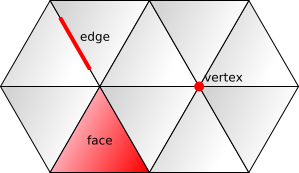
\includegraphics[scale=0.5]{kepek/img31.png}
\caption{A rácsok részei}
\label{fig:img31}
\end{figure}

\noindent A játékok nagy többségében közös az, hogy a rácsoknak csak az egyik részére koncentrálnak. A nyugati játékoknál mint a sakk vagy a dáma a rácsnak a lap részén van a fókusz ellentétben a keleti játékokkal mint a Go vagy a Csillaghalma (Chinese Checkers), ahol a csúcsokon van.
\newline
\newline Lapok, élek és csúcsok feltűnnek a különböző poligonokból álló  térképek esetén is. Egy olyan algoritmus ami a lapok, élek vagy csúcsok alapján működik de nincs szükség koordinátákra az működni fog ilyen térképek esetén is.

\begin{figure}[h]
\centering
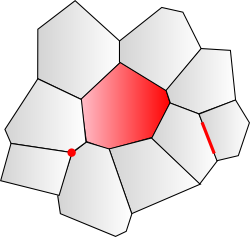
\includegraphics[scale=0.5]{kepek/img32.png}
\caption{Különböző poligonokból álló térkép.}
\label{fig:img32}
\end{figure}

\noindent A rácsok és a poligonális térképek átalakíthatóak gráf struktúrákra azáltal, hogy minden lapból csomópontot és minden lapok közötti élből pedig a csomópontok közötti gráf éleket készítünk. A gráf struktúra megengedi számunkra, hogy gráf algoritmusokat (például: legrövidebb út) használjunk a térképen.

\section*{Használatuk játékokban}

A számítógépes játékok mind a három típust használhatják, de a lap a leggyakoribb. Épületek, terület típusok (fű, sivatag, stb.) és a terület birtoklás a lapokat használja. Terület határok és az “áramlás” (“flow”) algoritmusok (ami szimulálja az áramlását a víznek, embereknek, termékeknek, stb. a szomszédos csempék között) használják az éleket. Az utakhoz lehet használni a lapokat és az éleket is.
\Chapter{Koordináta-rendszerek}

\section{Négyzet alapú rendszerek}

A négyzet alapú koordinátarendszer alatt jelen esetben a hagyományos \textit{Descartes-féle} koordinátarendszert értjük. Ennek a pontjait az $(x, y) \in \mathbb{Z}^2$ alakban írhatjuk föl.

% "A síkbeli \textit{Descartes-féle koordináta-rendszer}ben egy $P$ pont helyzetét az $XY$ síkon az $(x;y)$ rendezett számpárral (koordináta-kettős) adjuk meg. A két tengely metszéspontja a koordináta-rendszer kezdőpontja az origó $(O)$. A megállapodás szerinti első $x$ koordináta az abszcissza, a második $y$ koordináta az ordináta. Ugyanezekkel a jelzőkkel különböztetjük meg a tengelyeket. A vektoros értelmezésnél az $X$ és $Y$ tengelyek irányába mutató egységvektorokat $(i;j)$ jelöli." \cite{WikiSquare}

\section{Hexagon alapú rendszerek}
\label{sec:hexagon}

A hexagonok hat oldalú poligonok. A szabályos hatszögnek minden oldala egyenlő hosszúságú és belső szögei is egyenlőek. A szakdolgozatomban olyan hexagonokkal foglalkozok, amelyeknek a szemközti oldalai egyenlő hosszúságúak és párhuzamosak, viszont nem minden esetben feltétlenül szabályosak \cite{HexWiki}.

Egy hexagonnak hat oldala van. Minden oldalon két hexagon osztozik. Egy hexagonnak hat csúcsa van, minden csúcson 3 hexagon osztozik. A hexagonháló esetében többfajta megközelítés is szóbajöhet, most ezek közül fogok néhányat ismertetni.

A hexagonokból felépülő rácsokban a koordináták kezelésére többféle módszer is adódik. A következő szakaszokban ezeket veszem sorra, és hasonlítom össze.

\subsection{Eltolásos koordináta-rendszer}
% \cite{redblobgamesHexagonalGrids}

A leggyakoribb megközelítés a hexagon alapú rácsokban lévő koordináták kezeléséhez az eltolásos módszer, ami kisebb eltérésektől eltekintve gyakorlatilag megegyezik a \textit{négyzet koordináta-rendszer}rel. A \textit{négyzet koordináta-rendszer}hez hasonlóan itt is a hálónk egyik sarka lesz a kezdő pont (origó) amihez viszonyítva számozzuk majd a sorokat és az oszlopokat.

Az \textit{eltolásos koordináta-rendszer} egyik hátránya, hogy az egyik tengelye mentén nem egyenesen haladnak a sokszögek az eltolás miatt, és emiatt bonyolultabbá válnak a számítások (\ref{fig:OffsetCoord}. ábra). A további rendszerek ezt a problémát orvosolják, viszont ott más nehézségek merülnek fel.	

\begin{figure}[h!]
\centering
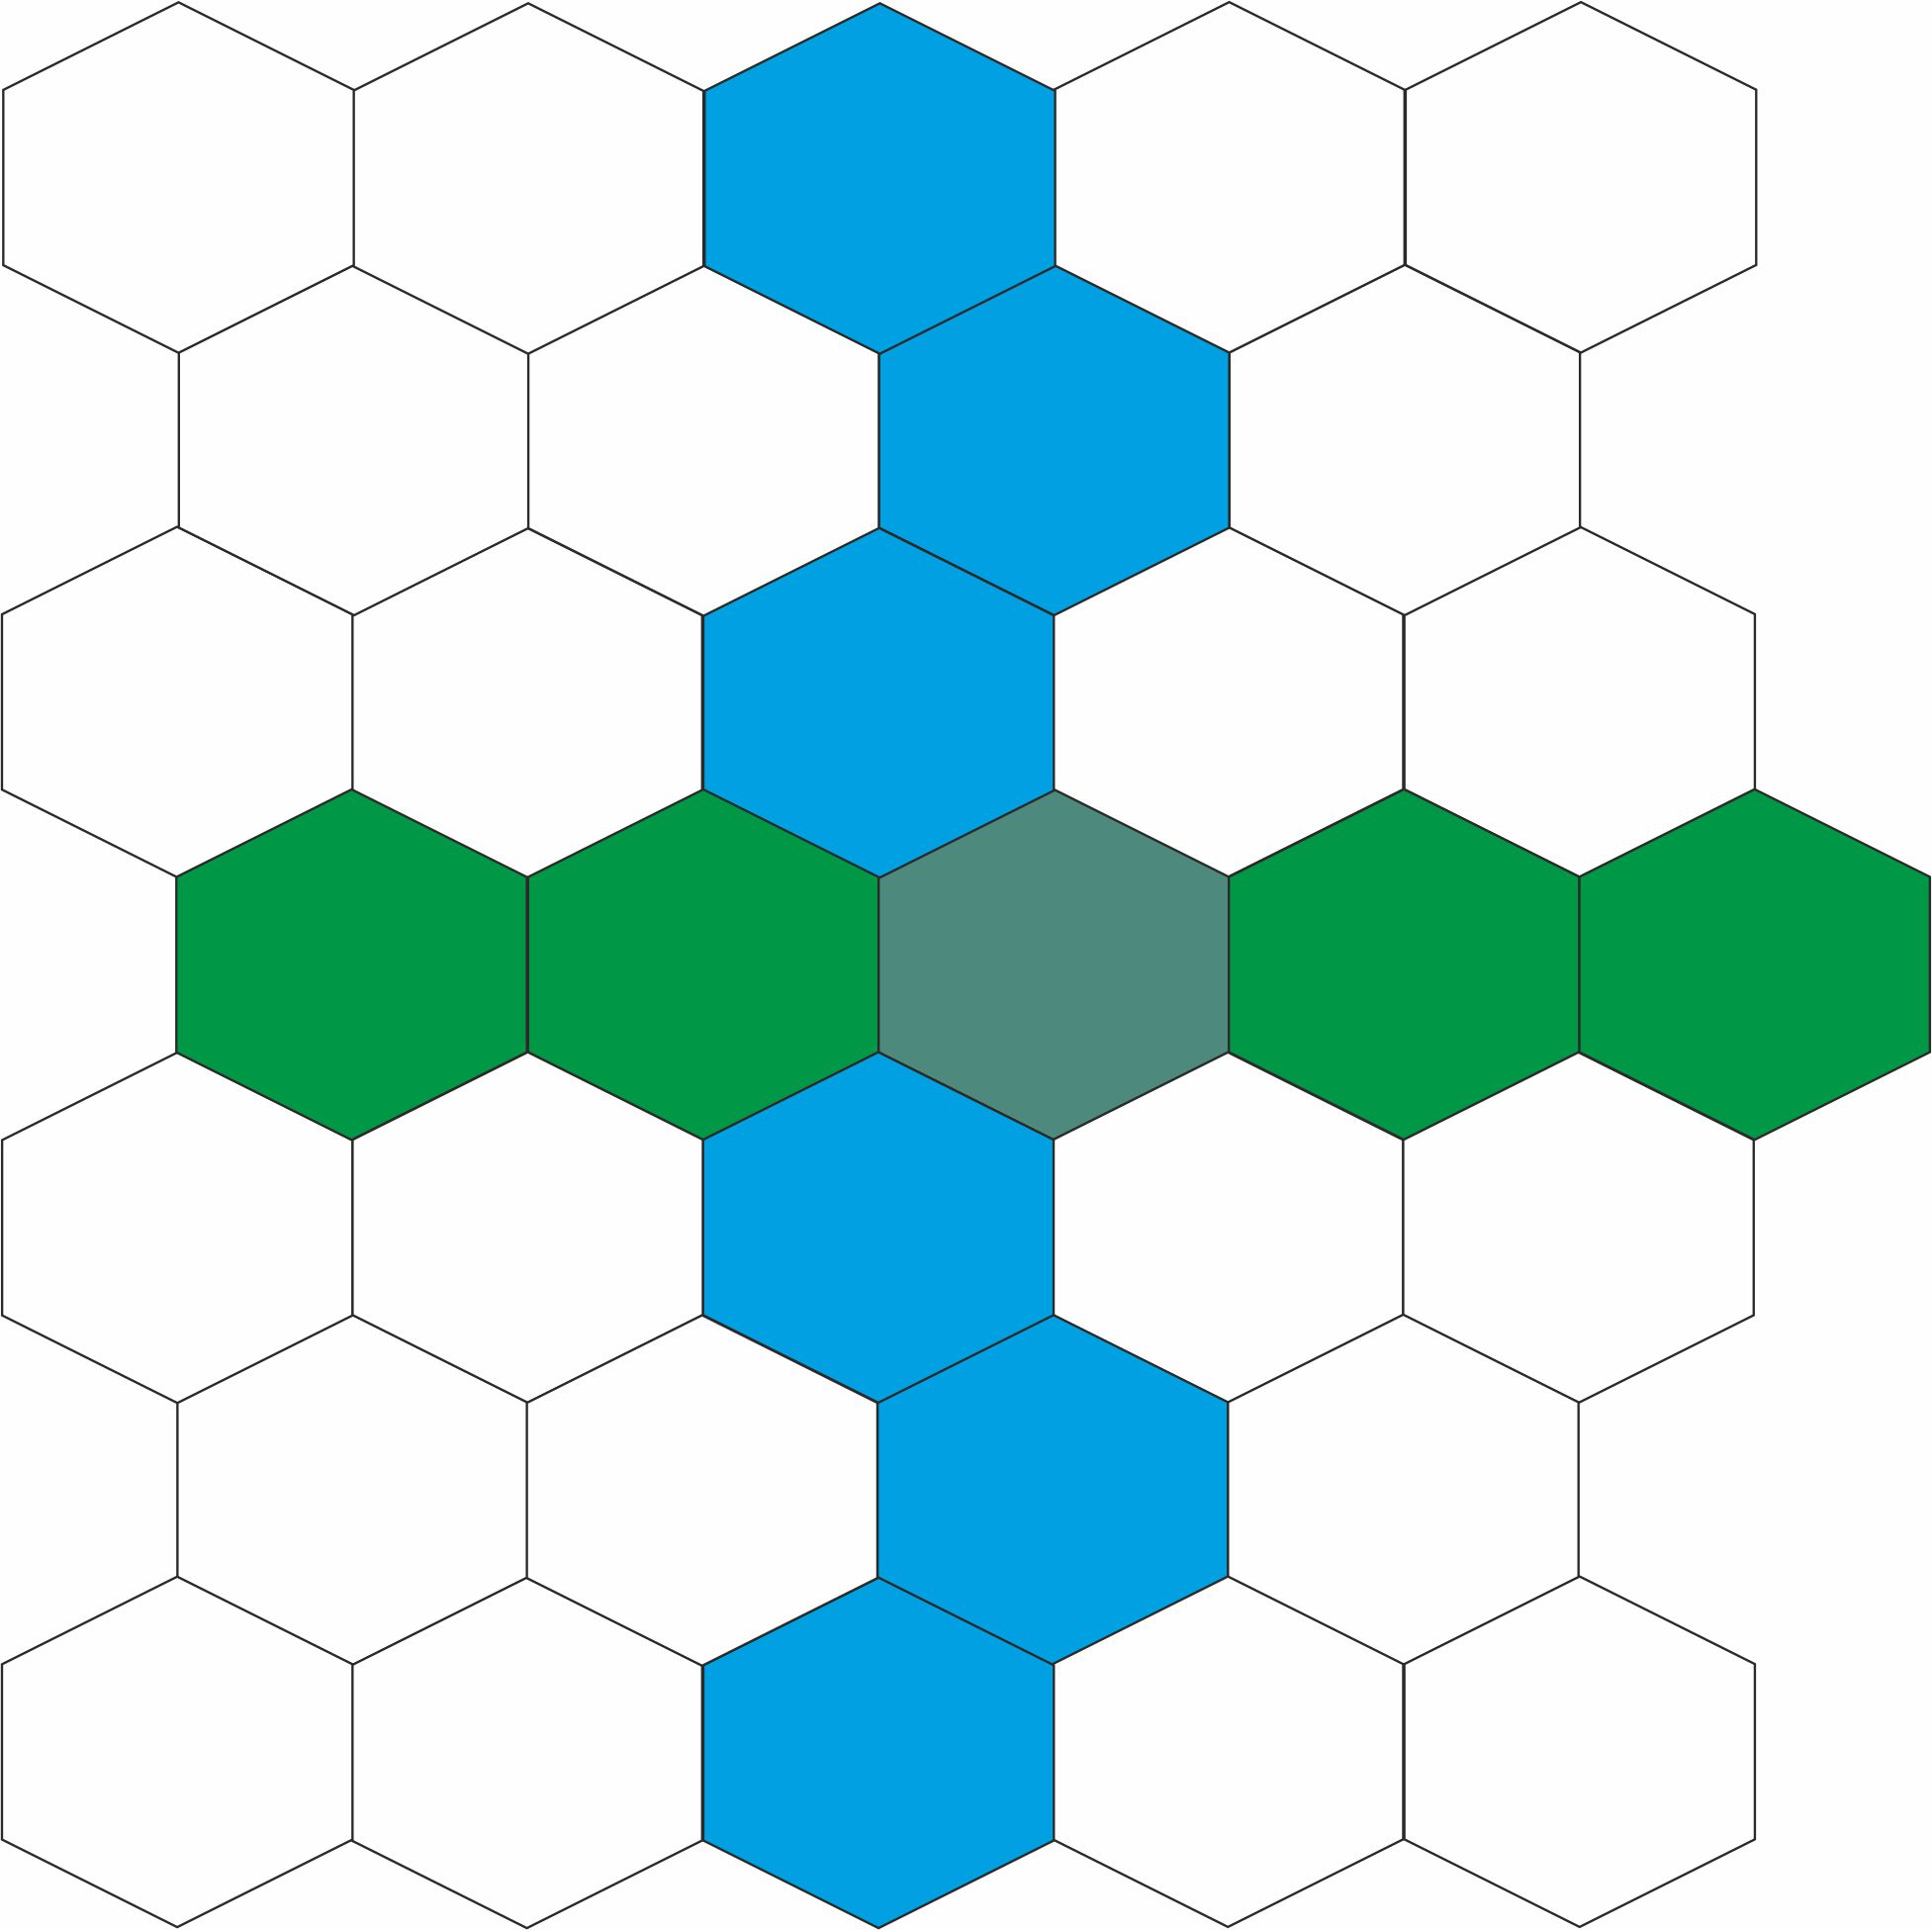
\includegraphics[scale=0.3]{kepek/OffsetCoord.jpg}
\caption{\textit{Eltolásos koordináta-rendszer}ben a tengelyek elhelyezkedése}
\label{fig:OffsetCoord}
\end{figure}

\newpage
A négyzethálóval is elérhetünk a hexagonhálóhoz hasonló hatást, ha a négyzethálóban minden páros/páratlan sort/oszlopot eltolunk (\ref{fig:Hex_Sq}. ábra).

\begin{figure}[h!]
\centering
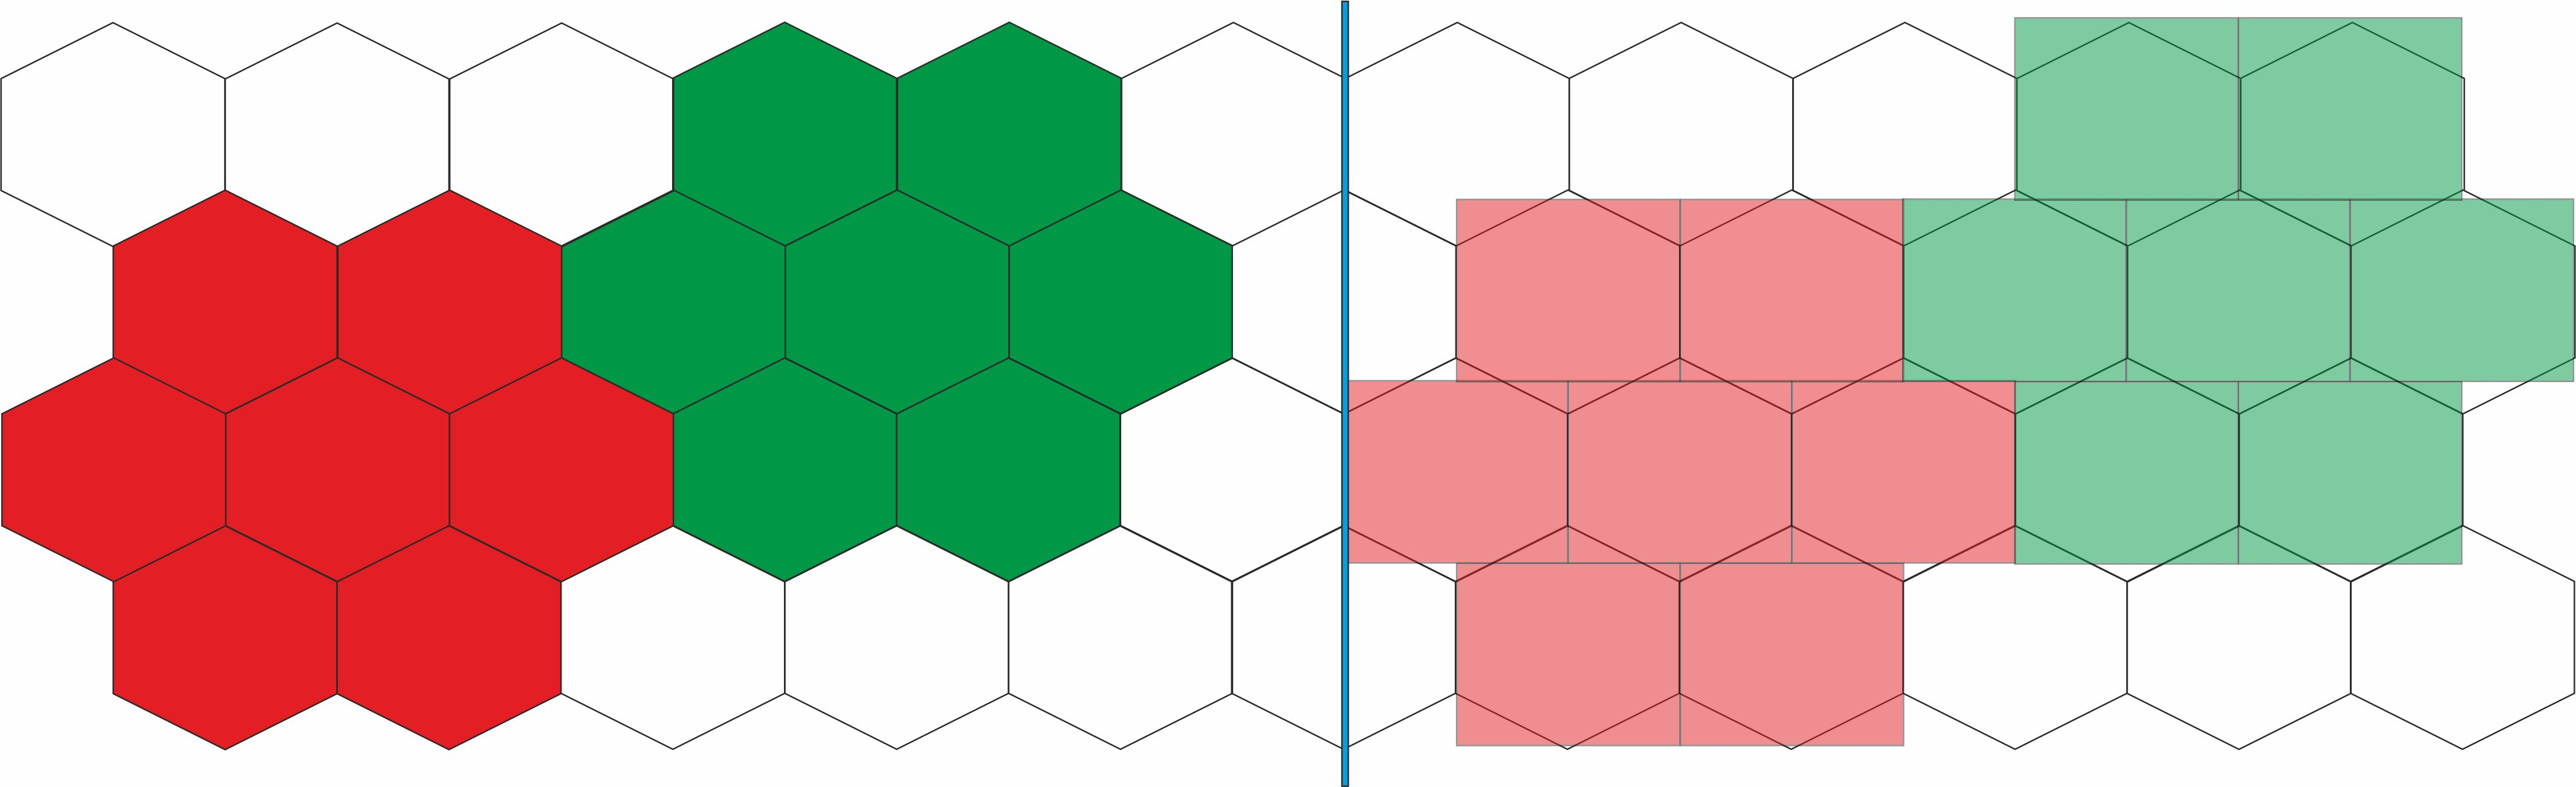
\includegraphics[scale=0.3]{kepek/Hex_Sq.jpg}
\caption{Hexagonrács az eltolt négyzetrácshoz viszonyítva}
\label{fig:Hex_Sq}
\end{figure}

Eltolható a páros és a páratlan oszlop/sor is. Mivel kétféleképpen is állhatnak a hexagonok, ezért négy fajta variáció érhető el összesen (\ref{fig:OffsetFour}. ábra) \cite{Offset}.

\begin{figure}[h!]
\centering
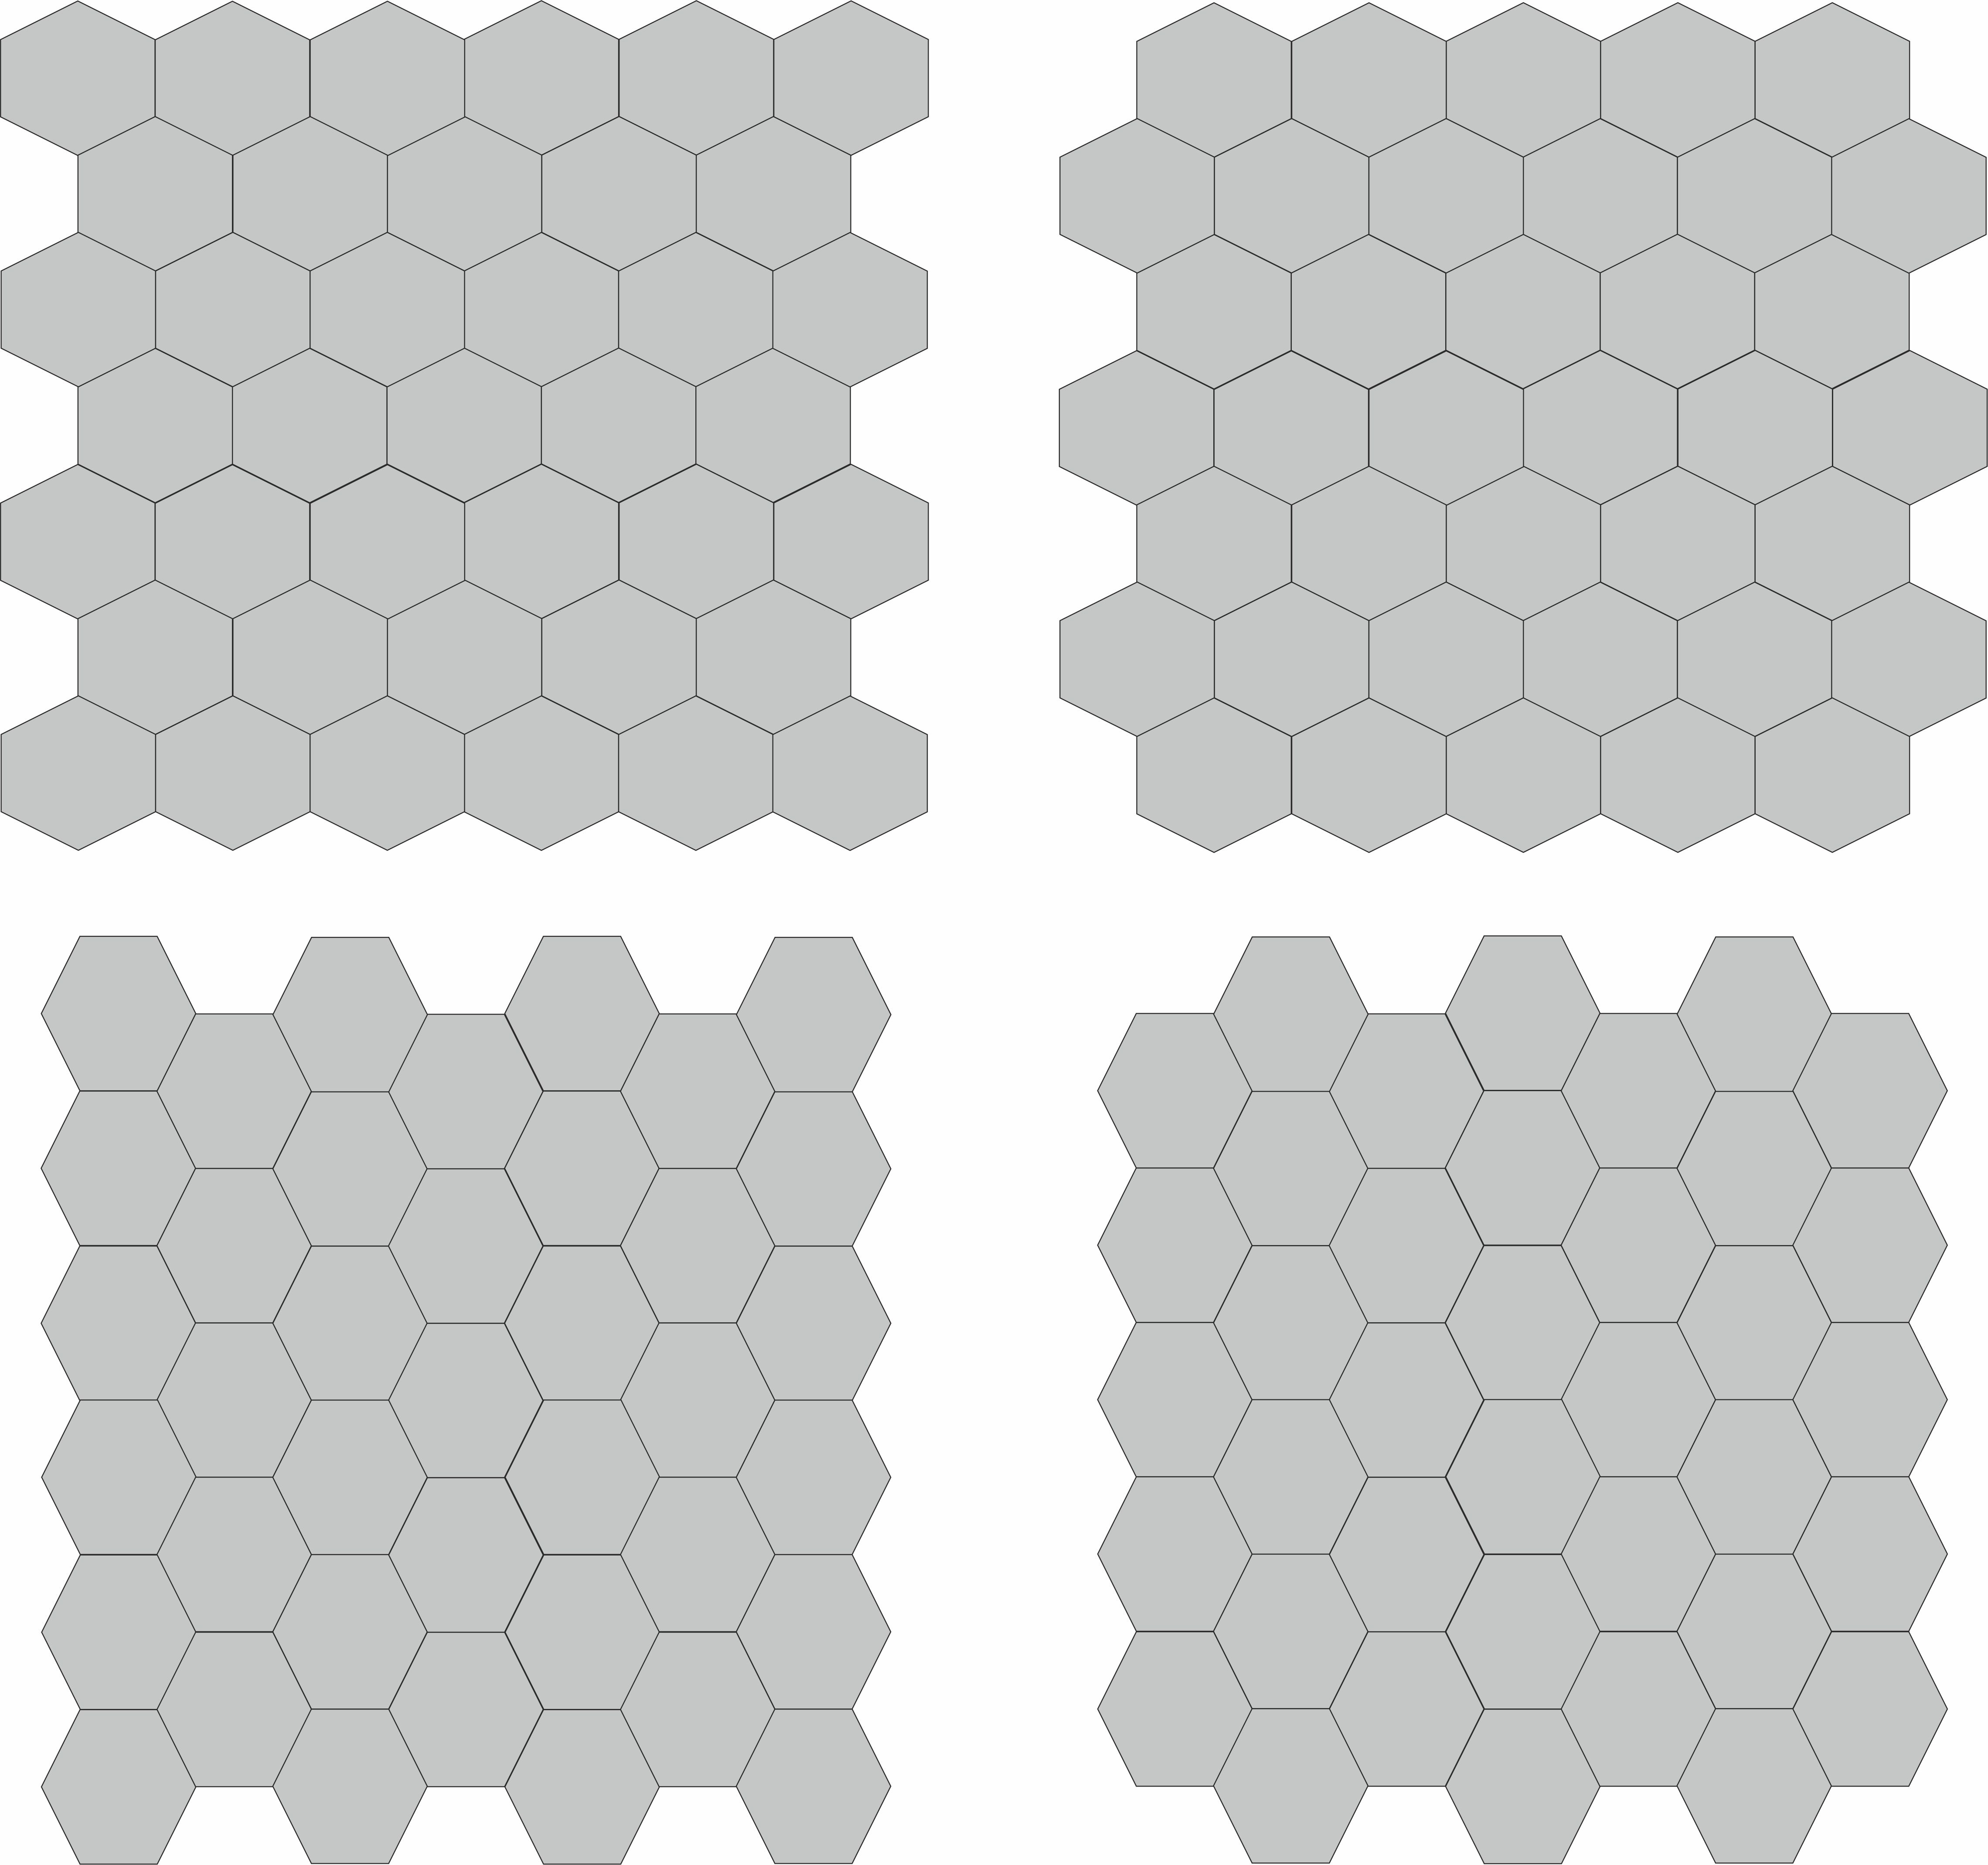
\includegraphics[scale=0.2]{kepek/OffsetFour.jpg}
\caption{A négyféle ábrázolási mód}
\label{fig:OffsetFour}
\end{figure}

\newpage
\subsection{Kocka koordináta-rendszer}
%\cite{redblobgamesHexagonalGrids}

Ha egy másik fajta megközelítésből nézzük a hexagon hálókat, akkor láthatjuk, hogy három elsődleges tengelye van, nem úgy mint a korábbi koordináta-rendszereknek (\ref{fig:CubeCoord}. ábra).

\begin{figure}[h!]
\centering
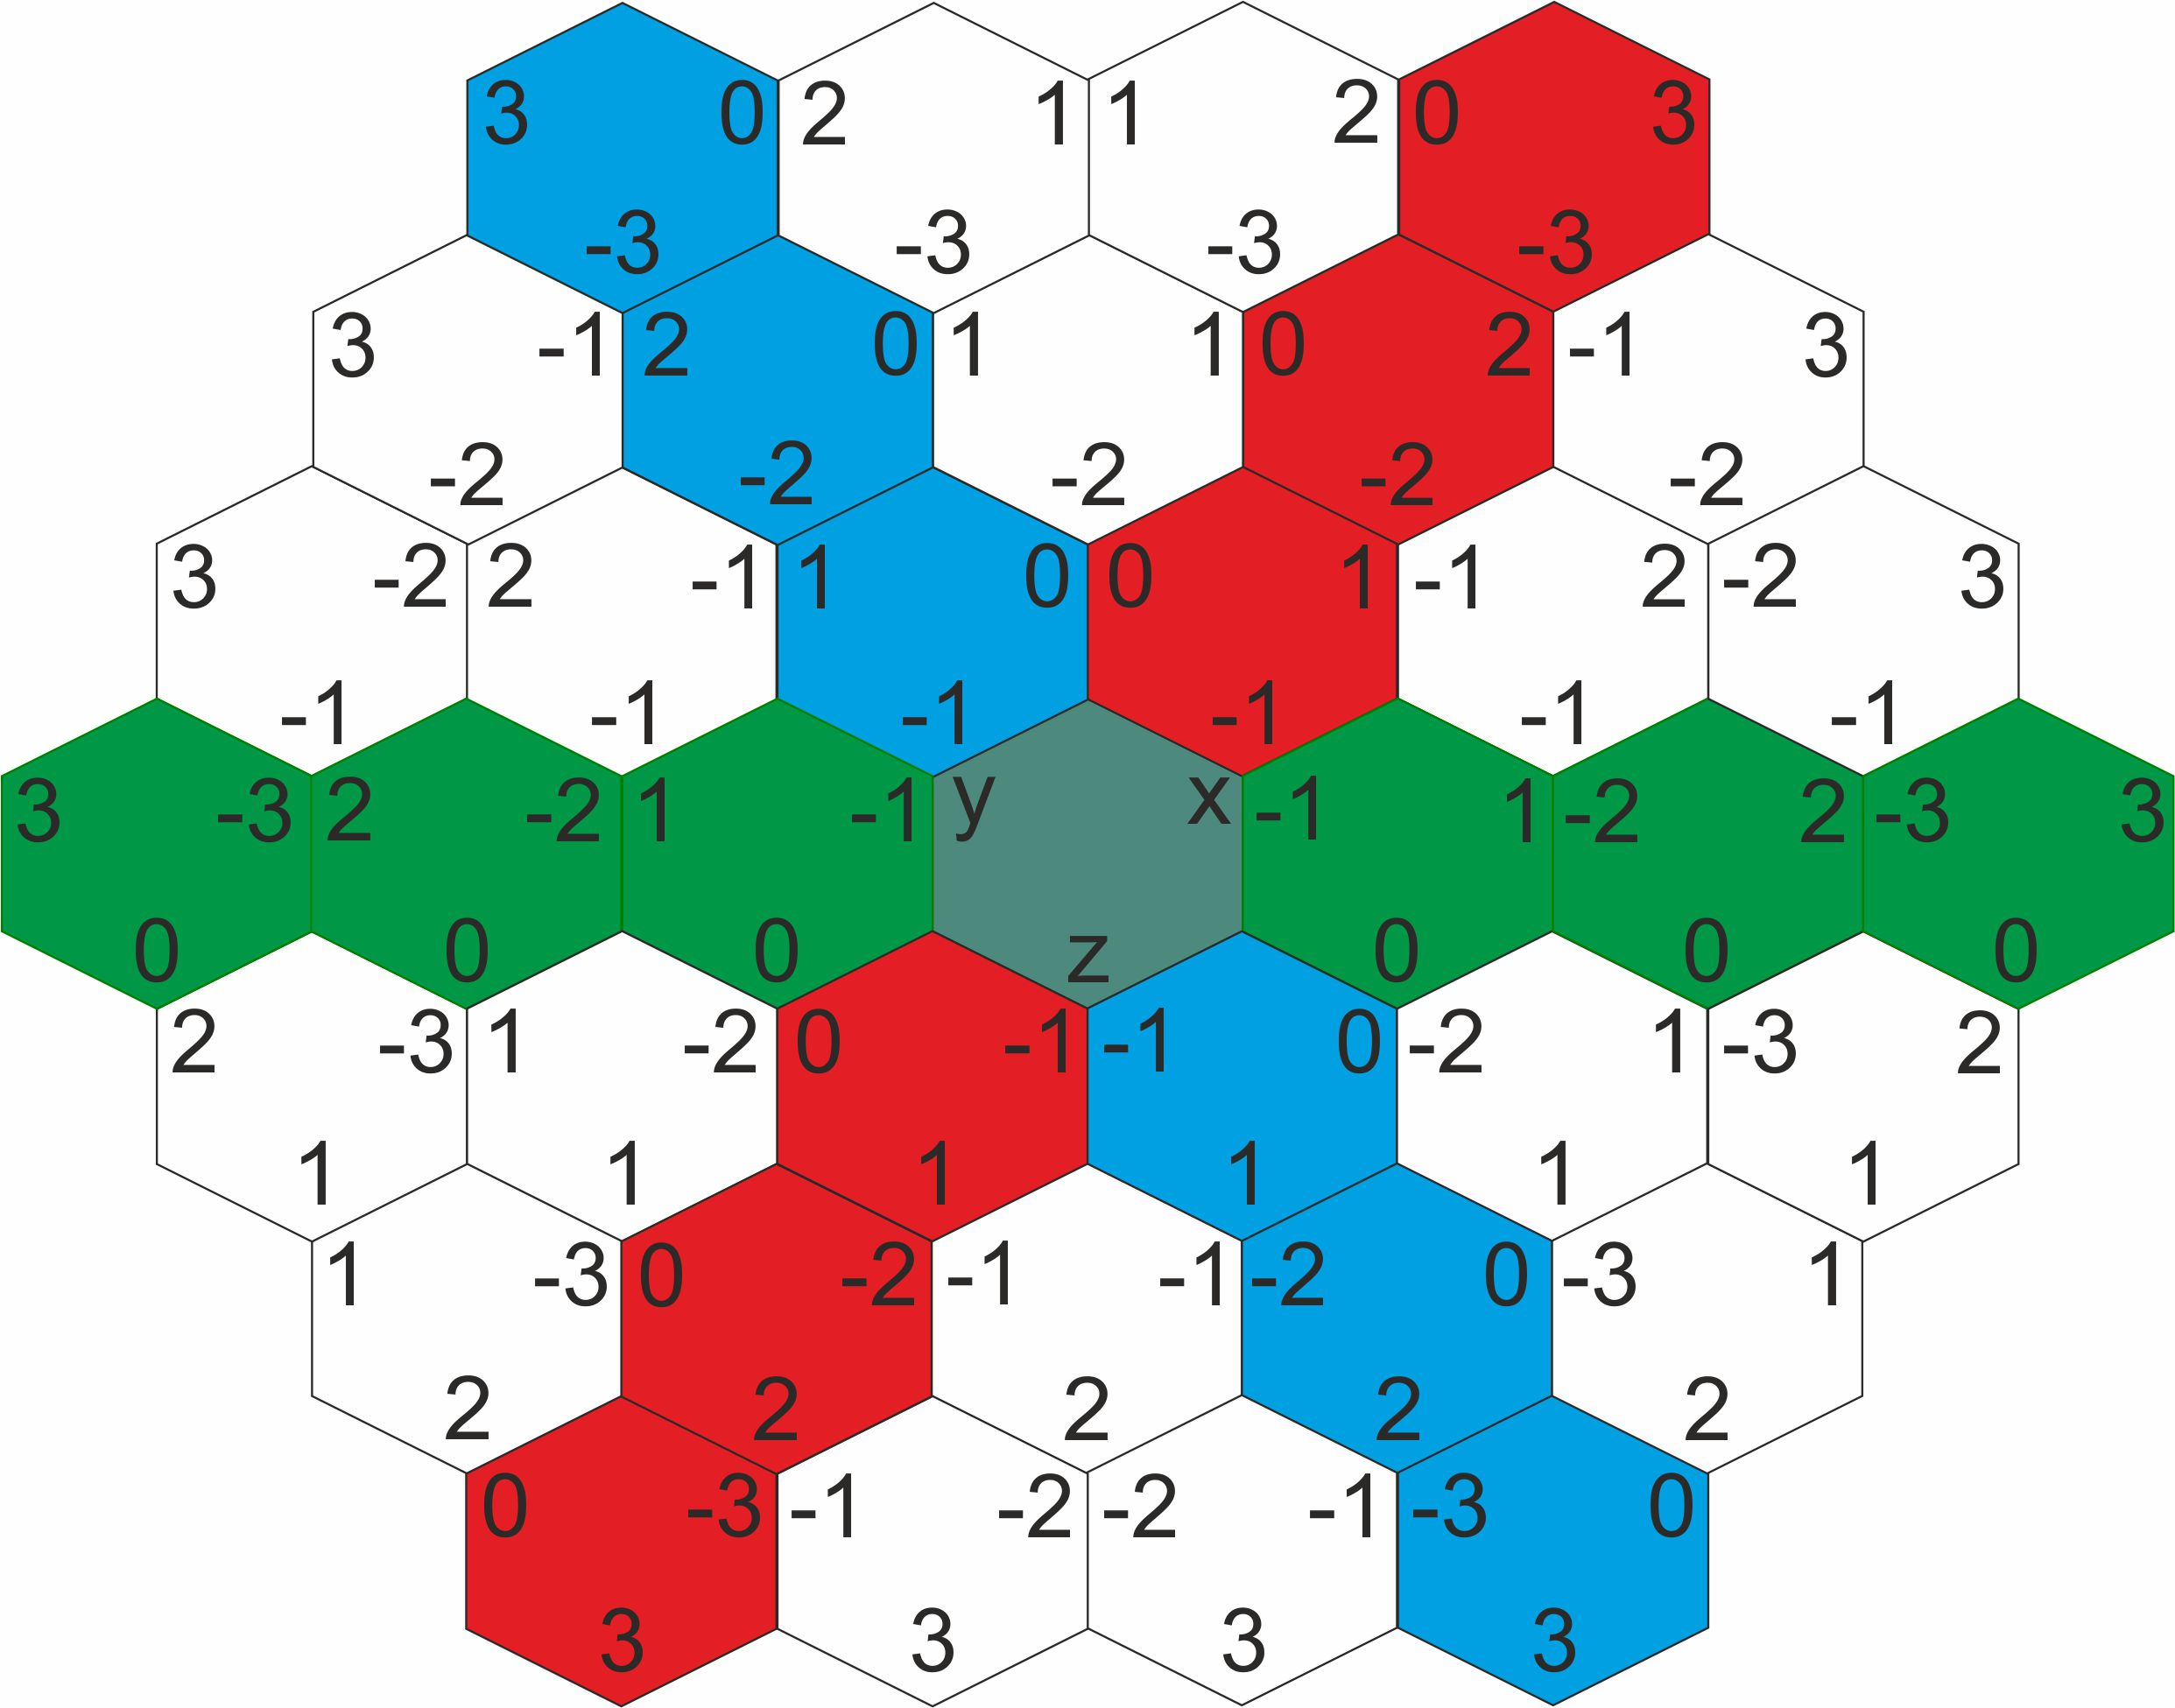
\includegraphics[scale=0.4]{kepek/CubeCoord.jpg}
\caption{A \textit{kocka koordináta-rendszer}ben a tengelyek elhelyezkedése}
\label{fig:CubeCoord}
\end{figure}

Ahhoz, hogy megértsük a \textit{kocka koordináta-rendszer}t képzeljünk el egy kockarácsot és vágjunk ki belőle egy átlós síkot az $x + y + z = 0$ mentén. Ez fogja majd a hexagonrácson használt algoritmusokat egyszerűbbé tenni azáltal, hogy használhatjuk a \textit{Descartes-féle koordináta-rendszer}ben való műveleteket. Ilyen műveletek az eltolás hozzáadása vagy kivonása a  koordinátákból, szorzás vagy osztás skalárral, távolság számítása.

Egy szemléletesebb példaként vizsgáljuk meg a \textit{Q*bert} nevű játékot (\ref{fig:Qbert}. ábra).

\begin{figure}[h!]
\centering
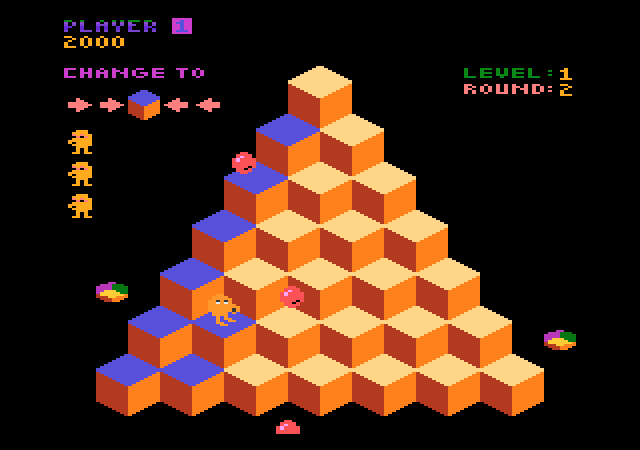
\includegraphics[scale=0.5]{kepek/Qbert.png}
\caption{A \textit{Q*bert} című játék}
\label{fig:Qbert}
\end{figure}

A játék egy $28$ kockából álló, piramis szerű játékmezőn zajlik. (Ilyen alakzatot kapunk, ha végrehajtjuk az előző részben leírt síkkal való vágást.) \newpage \noindent A játékos \textit{Q*bert}-et (narancssárga karakter) irányítja, aki, ha ráugrik egy kockára akkor átszínezi azt. Ha jobban megfigyeljük az ábrát, akkor láthatjuk, hogy a kockák valójában hexagonok, ha síkba rajzoljuk le. Így tehát \textit{Q*bert} 6 különböző irányba is léphet. Ez azt jelenti, hogy ha a párhuzamosan lévő oldalakra merőlegesen helyezünk tengelyeket, akkor hármat tudunk elhelyezni 120 fokonként. Vegyük észre az alábbiakat \cite{HexagonalGrids}.
\begin{itemize}
\item Minden hexagonnak 3 koordinátája van. 
\item Mindegyik tengely egy egyenes vonalnak felel meg a hexagon hálón.
\item Minden irány a hexagonon másik két iránynak a kombinációja a \textit{kocka koordináta-rendszer}en. Például, ha a \ref{fig:Qbert}. ábrán felfelé szeretnénk mozogni, akkor az a $+y$ és $-z$ között fekszik, ezért minden lépésnél ami felfelé történik hozzá kell adnunk 1-et az $y$-hoz és el kell vennünk 1-et a $z$-ből. 
\end{itemize}
Ez azért történik így, mert minden egyes mező koordinátájának az összege $0$ kell, hogy legyen ($x + y + z = 0$). Ez azt is jelenti, hogy a harmadik tengely bizonyos esetekben redundáns is lehet, például amikor meghatározzuk, hogy az egyes mezők hol jelenjenek meg a képernyőn. Ugyanakkor olyan esetekben amikor algoritmusokat (útkereső algoritmus) kell használni az előnye egyértelműen látszik (az algoritmusok könnyebb használhatósága miatt) \cite{Cube}. 

\subsection{Tengely koordináta-rendszer}

A \textit{tengely koordináta-rendszer} csak két koordinátát használ a \textit{kocka koordináta-rendszer} három koordinátája közül (\ref{fig:AxialCoord}. ábra). Mivel a \textit{kocka koordináta-rendszer}nél szükségszerű, hogy  $x + y + z = 0$ teljesüljön, a harmadik koordináta redundáns.  A \textit{tengelyes koordináta-rendszer} használható tárolásra és megjelenítésre, mivel az $x + y + z = 0$ egyenlet alapján kiszámítható a harmadik koordináta ezért a számításokhoz is könnyen használható \cite{Axial}.

\begin{figure}[h!]
\centering
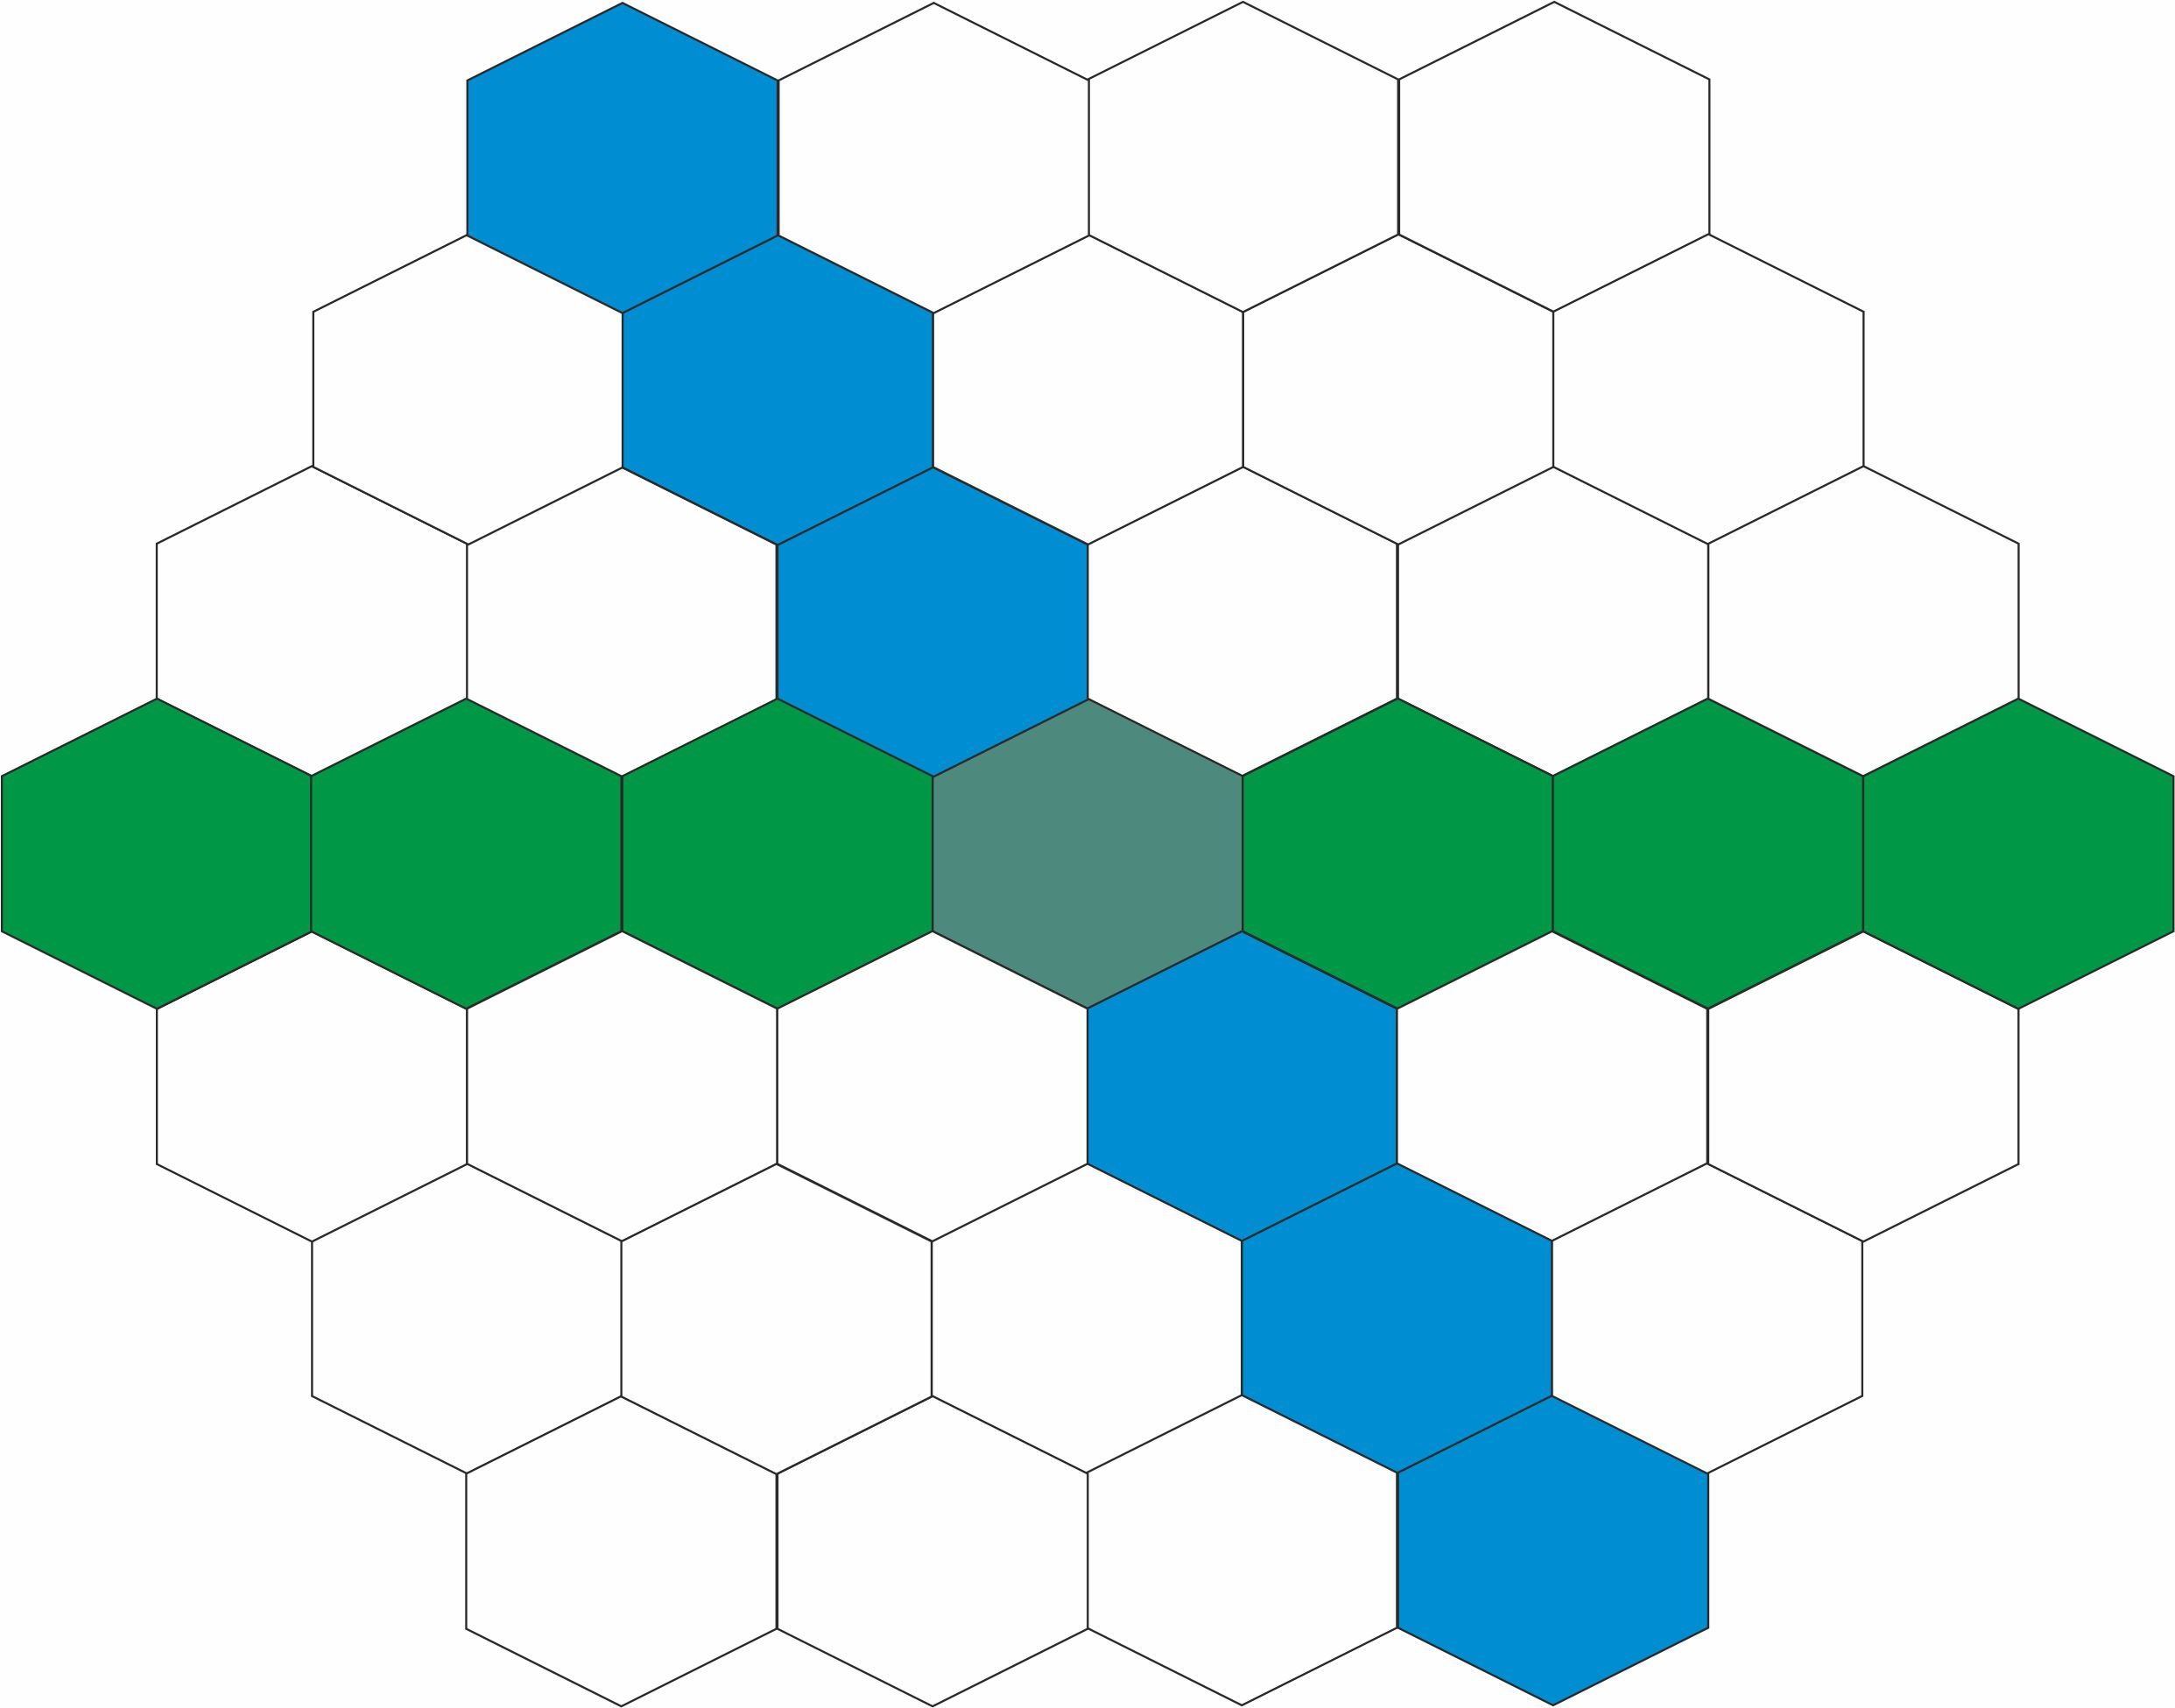
\includegraphics[scale=0.3]{kepek/AxialCoord.jpg}
\caption{A \textit{tengely koordináta-rendszer}ben a tengelyek elhelyezkedése}
\label{fig:AxialCoord}
\end{figure}

Az előnye ennek a rendszernek az eltolásoshoz képest, hogy az algoritmusok egyszerűbbek. A hátránya viszont a téglalap alakú térképek esetén való tárolás. 

\newpage
\section{Térkép tárolási probléma}
% \cite{redblobgamesHexagonalGrids}

A megjelenítő eszközeink néhány ritka kivételtől eltekintve téglalap alakúak. A számítógépes játékok jelentős része szintén téglalap alakú elrendezésekben gondolkozik. A számítógép az adatokat lineáris elrendezésben képes tárolni. A problémát az jelenti, hogy az indexeket hogyan számoljuk át úgy, hogy lehetőleg hézagmentesen tudjuk tárolni az egyes koordinátákhoz tartozó adatokat.

Síkbeli elrendezés esetén két koordináta elegendő a pozíciók egyértelmű meghatározásához. Ebből adódik, hogy a programozási nyelvekben használt mátrixos elrendezésből induljunk ki.

A következőkben annak a részletezésére kerül sor, hogy hogyan tudjuk a lehető legkevesebb kompromisszummal illeszteni a hatszög alapú elrendezésünket a kétdimenziós mátrixokhoz használt tárolási móddal.

\begin{figure}[h!]
\centering
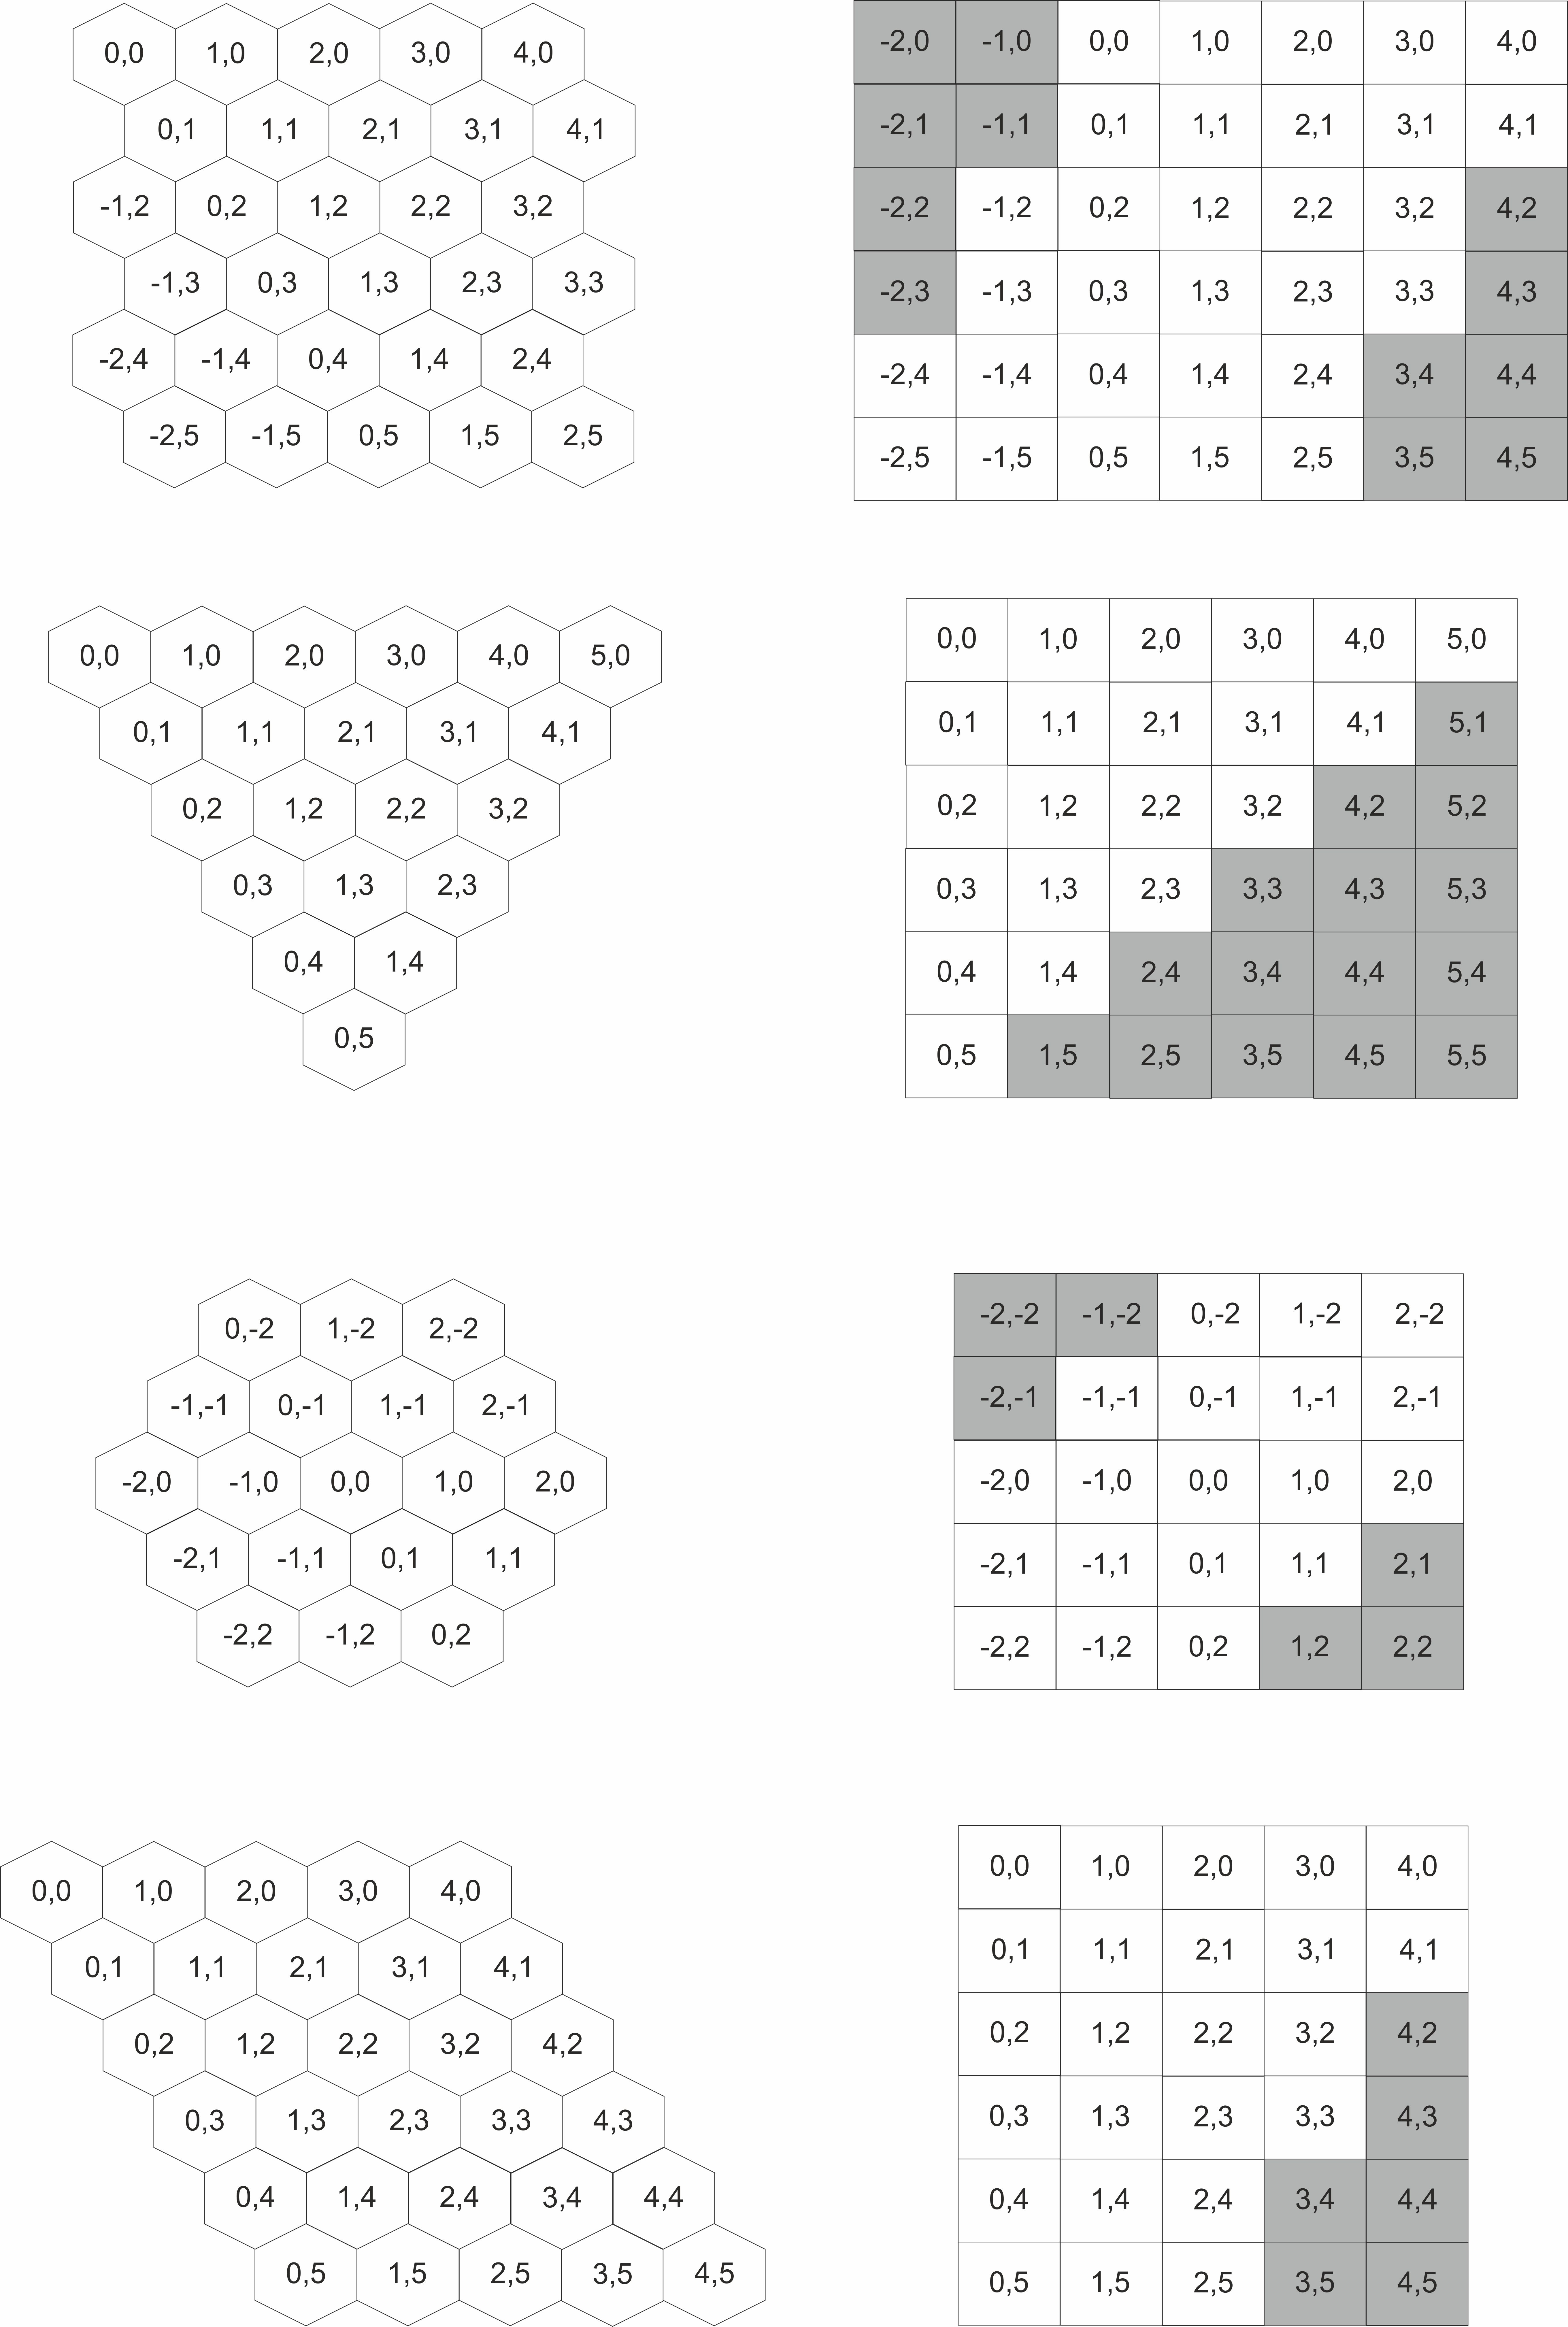
\includegraphics[scale=0.235]{kepek/StorageProblem.jpg}
\caption{Bal oldalt a különböző alakú térképek, jobb oldalt pedig a hozzájuk tárolt adat látható.}
\label{fig:StorageProblem}
\end{figure}

\noindent Vegyük észre a \ref{fig:StorageProblem}. ábrán látható képeken, hogy az elpazarolt hely a sorok bal és jobb szélén jelentkezik (kivéve a rombusz esetén). Az egyes cellákban a számpárok a $(q, r)$ oszlop és sor indexet jelölik. A hagyományos, \textit{sor-oszlop} sorrend helyett az indexelésnél az \textit{oszlop-sor} szerepel, mert a képi koordináta-rendszerekben $(x, y)$ tengely esetén ilyen sorrendben szokták használni \cite{Storage}.

Három lehetséges megoldás létezik a probléma kiküszöbölésére.
\begin{itemize}
\item Hagyjuk figyelmen kívül a problémát. Használjunk mátrixot a tárolásra és használjunk valamilyen speciális jelzőt a nem létező mezőkre. A legtöbb esetben nem éri meg ennél komplikáltabb megoldást alkalmazni.
\item Használjunk valamilyen listát a mezőkről a mátrix helyett. Ezáltal lehetőségünk lesz szabálytalan formájú térképek készítésére, beleértve azt is, hogy legyen egy lyuk a közepén. A rács osztályból \textit{getter/setter} metódusok segítségével könnyen el lehet érni (például \texttt{Grid(Tile(x, y)))}).
\item Csúsztassuk el a sorokat úgy, hogy bal oldalt ne legyen “üres” hely. Néhány nyelvben a kétdimenziós tömb az egy tömbökből álló tömb, ilyen esetekben a tömböknek nem kell egyforma hosszúaknak lenniük, így eltüntethető a felesleg a jobb oldalról is. Amennyiben egy olyan, szabálytalan alakú térképről van szó, amelynél a sorok hossza nem számítható, akkor érdemes a sorok első elemének indexeit egy külön tömbben letárolni. Ezen tömb $i$-edik elemét jelölje $a_i$. Ekkor a $q$-adik sor $r$-edik oszlopát ($0$-tól kezdődő indexet feltételezve) az $a_q + r$ címen találjuk.
\end{itemize}

Szabályos alakú térképek esetén az indexek közvetlenül számolhatók.
\begin{itemize}
\item A téglalap alakú térképek esetén az eredeti hexagonális $(q, r)$ koordinátákhoz a sorok kezdőindexeit az
$$
a_r = - \left\lfloor \dfrac{r}{2} \right\rfloor
$$
összefüggéssel számíthatjuk ki. Ez tulajdonképpen az eltolásos koordináta-rend\-szer\-be való konverziót jelenti. (A negatív index azért nem jelent problémát, mert azon $r$ értékek kerülnek levágásra, ahol az összeg negatív lenne.)
\item A háromszög alakú térképek esetén alsó- vagy felsőháromszög tárolási módot használhatunk. Alsóháromszög esetén a kezdőindexeket az
$$
a_r = \dfrac{q \cdot (q + 1)}{2}
$$
formában számíthatjuk.
\item Tekintsünk egy $N$ sugarú ($N - 1$ maximális indexekkel rendelkező) hatszög alakú térképet, ahol az origó a hatszög közepén van. Külön kell vizsgálnunk a sorindex előjelének megfelelően két esetet.

Tegyük fel, hogy $r \leq 0$. Ekkor $r$ indexű sorhoz tartozó kezdőcímet az
\begin{align*}
a_r &=
\dfrac{
(2N - 2 + r)(2N - 1 + r)
}{2}
-
\dfrac{
N(N - 1)
}{2} \\
&=
\dfrac{r^2 + (4N - 3)r + (3N^2 - 5N + 2)}{2}
\end{align*}
formában számíthatjuk ki, a címet pedig az $a_r + (N - 1 -r) + q$ alakban.

Az $r > 0$ esetben a számítást az
\begin{align*}
a_r &=
\dfrac{2N(2N - 1)}{2} -
\dfrac{(2N - r - 1)(2N - r)}{2} +
\dfrac{(2N - 1)(2N - 2)}{2} -
\dfrac{N(N - 1)}{2} \\
&=
\dfrac{-r^2 + (4N - 1)r + (3N^2 - 5N + 2)}
{2}
\end{align*}
összefüggés írja le. A $(q, r)$ koordinátájú elem indexe ekkor $a_r + (N - 1 + r) + q$ értékével lesz egyenlő.
\item A rombusz formájú térkép esetén minden tökéletesen egyezik, ezért egyszerűen csak az $a_r = 0$ kezdőindexekkel kell számolnunk.
\end{itemize}

\section{Koordináta konverziók}

Mivel a három terület ahol a koordinátákat használjuk (tárolás, megjelenítés, számítások) nem feltétlenül ugyanabban a koordináta-rendszerben fognak megvalósulni, ezért szükséges ismernünk a különböző konverziós eljárásokat oda-vissza a különböző rendszerek között. Mivel a számításokhoz a \textit{kocka koordináta-rendszer}t fogom alkalmazni, ezért erre a rendszerre fogom alapozni az algoritmusokat \cite{Conversion}.

\subsection{Tengely - Kocka konverziók}
% \cite{redblobgamesHexagonalGrids}

A \textit{tengely koordináta-rendszer} nagyon közel áll a \textit{kocka koordináta-rendszer}hez. A tengelyes csak elhagyja a harmadik koordinátát, a kocka pedig kiszámolja a harmadikat a másik kettő alapján \cite{Conv_Axial}.

%\begin{verbatim}
%function cube_to_axial(cube):
%    var q = cube.x
%    var r = cube.z
%    return Hex(q, r)
%function axial_to_cube(hex):
%    var x = hex.q
%    var z = hex.r
%    var y = -x-z
%    return Cube(x, y, z)
%\end{verbatim}

\begin{align*}
axial_{q, r}(cube_{x}, cube_{y}) &=
\left(
\begin{array}{c}
cube_{x} \\
cube_{y}
\end{array}
\right)
\\
cube_{x,y,z} (axial_{q}, axial_{r}) &=
\left(
\begin{array}{c}
axial_q \\
axial_r \\
-axial_q - axial_r
\end{array}
\right)
\end{align*}

\subsection{Eltolásos - Kocka konverziók}
% \cite{redblobgamesHexagonalGrids}

Az \textit{eltolásos koordináta-rendszer}nek négy fajta típusa lehet az alapján, hogy melyik sor/oszlop lett eltolva. A páratlan indexű sorok eltolása esetén a következő formában számítható az összefüggés \cite{Conv_Offset}.
\begin{align*}
&oddrow_{row, col}(cube_{x},cube_{z}, cube_{z}) =
\left(
\begin{array}{c}
cube_{x} + \dfrac{cube_{z} - (cube_{z} \bmod 2)}{2} \\
cube_{z}
\end{array}
\right),
\\
&cube_{x, y, z}(oddrow_{row}, oddrow_{col}) =
\left(
\begin{array}{c}
oddrow_{col} - \dfrac{oddrow_{row} - (oddrow_{row} \bmod 2)}{2} \\
oddrow_{row} \\
-cube_{x} - cube_{y}
\end{array}
\right)
\end{align*}

%\begin{verbatim}
%function cube_to_oddr(cube):
%      col = cube.x + (cube.z - (cube.z&1)) / 2
%      row = cube.z
%      return Hex(col, row)
%
%function oddr_to_cube(hex):
%      x = hex.col - (hex.row - (hex.row&1)) / 2
%      z = hex.row
%      y = -x-z
%      return Cube(x, y, z)
%\end{verbatim}

A páros indexű sorok eltolása esetén a következő módon számíthatjuk az indexeket.
\begin{align*}
&evenrow_{row, col}(cube_{x}, cube_{z}) =
\left(
\begin{array}{c}
cube_{z} \\
cube_{x} + \dfrac{cube_{z} + (cube_{z} \bmod 2)}{2} \\
\end{array}
\right),
\\
&cube_{x, y, z}(evenrow_{row}, evenrow_{col}) = \\
&\left(
\begin{array}{c}
evenrow_{col} - \dfrac{evenrow_{row} + (evenrow_{row} \bmod 2)}{2} \\
-cube_{x} - cube_{z} \\
evenrow_{row} \\
\end{array}
\right)
\end{align*}


%\begin{verbatim}
%function cube_to_evenr(cube):
%      col = cube.x + (cube.z + (cube.z&1)) / 2
%      row = cube.z
%      return Hex(col, row)
%
%function evenr_to_cube(hex):
%      x = hex.col - (hex.row + (hex.row&1)) / 2
%      z = hex.row
%      y = -x-z
%      return Cube(x, y, z)
%\end{verbatim}

Páratlan indexű oszlop eltolásakor a számítás:

\begin{align*}
&oddcolumn_{row, col}(cube_{x}, cube_{z}) =
\left(
\begin{array}{c}
cube_{z} + \frac{cube_{x} - (cube_{x} \bmod 2)}{2} \\
cube_{x} \\
\end{array}
\right),
\\
&cube_{x,y,z} (oddcolumn_{row}, oddcolumn_{col}) = \\
&\left(
\begin{array}{c}
oddcolumn_{col} \\
-cube_{x} - cube_{z} \\
oddcolumn_{row} - \dfrac{oddcolumn_{col} - (oddcolumn_{col} \bmod 2)}{2} \\
\end{array}
\right).
\end{align*}

%\begin{verbatim}
%function cube_to_oddq(cube):
%      col = cube.x
%      row = cube.z + (cube.x - (cube.x&1)) / 2
%      return Hex(col, row)
%
%function oddq_to_cube(hex):
%      x = hex.col
%      z = hex.row - (hex.col - (hex.col&1)) / 2
%      y = -x-z
%      return Cube(x, y, z)
%\end{verbatim}

Utolsó esetként a páros indexű oszlopokkal való eltolás számítása a következő:

\begin{align*}
&evencolumn_{row, col}(cube_{x}, cube_{z}) =
\left(
\begin{array}{c}
cube_{z} + \frac{cube_{x} + (cube_{x} \bmod 2)}{2} \\
cube_{x} \\
\end{array}
\right),
\\
&cube_{x,y,z}(evencolumn_{row}, evencolumn_{col}) = \\
&\left(
\begin{array}{c}
evencolumn_{col} \\
-cube_{x} - cube_{z} \\
evencolumn_{row} - \dfrac{evencolumn_{col} + (evencolumn_{col} \bmod 2)}{2}
\end{array}
\right).
\end{align*}

%\begin{verbatim}
%function cube_to_evenq(cube):
%      col = cube.x
%      row = cube.z + (cube.x + (cube.x&1)) / 2
%      return Hex(col, row)
%
%function evenq_to_cube(hex):
%      x = hex.col
%      z = hex.row - (hex.col + (hex.col&1)) / 2
%      y = -x-z
%      return Cube(x, y, z)
%\end{verbatim}

Az implementációban érdemes \textit{bitenkénti “és”} (\texttt{a \& 1}) operátort használni \textit{modulo} (\texttt{a \% 2}) helyett, amikor meghatározzuk, hogy páros vagy páratlan sorban/oszlopban vagyunk, mivel ez működik negatív számok esetén is, függetlenül a maradékképzés műveletének programnyelvi implementálási módjától.

\newpage
\section{Távolságok számítása}
\label{sec:tavolsag}

Ahhoz, hogy távolságokat tudjunk számolni a térképen definiálnunk kell hozzá metrikákat. A különböző típusú koordináta-rendszerek esetén ennek különféle módjai lehetnek. A következő szakaszok ezek közül mutatnak be néhányat \cite{Distance}.

\subsection{Kocka koordináta-rendszer}
% \cite{redblobgamesHexagonalGrids}

A \textit{kocka koordináta-rendszer}ben, minden hexagon egy kockának felel meg a három dimenziós térben. A szomszédos hexagonok 1 távolságra vannak egymástól a hexagonháló esetén, viszont 2 távolságra vannak egymástól a \textit{kocka koordináta-rendszer}ben. Ezáltal egyszerűbbé válik a távolságszámítás.

Jelölje $dx$ az $x$ tengely irányú különbségeket, a $dy$ és $dz$ pedig hasonlóképp az $y$ és $z$ tengelyek esetében. A \textit{négyzet koordináta-rendszer} esetén a \textit{Manhattan-távolság} távolság az $|dx| + |dy|$ formában írható föl. Ugyanez \textit{kocka koordináta-rendszer}ben $|dx| + |dy| + |dz|$. Ezekből következik, hogy a hexagonrács esetén a \textit{Manhattan-távolság} a kockarács esetén fennálló távolság fele, vagyis
$$
d_{\text{cube}}(a, b) =
\dfrac{|a_x - b_x| + |a_y - b_y| + |a_z - b_z|}{2}.
$$

Egy ezzel egyenértékű megközelítés az is, ha megfigyeljük azt, hogy a három koordináta közül az egyiknek mindenképpen a másik kettő összegének kell lennie. Ekkor az az egy lesz a távolság \cite{Distance_Cube}:
$$
d_{\text{cube}}(a, b) =
\max(
|a_x - b_x|, |a_y - b_y|, |a_z - b_z|
).
$$

\subsection{Tengelyes koordináta-rendszer}
%\cite{redblobgamesHexagonalGrids}
%\cite{HexagonalGrids}

A \textit{tengelyes koordináta-rendszer}ben a számításokhoz szükséges három koordinátából kettőt ismerünk, ezért konvertálnunk kell majd a \textit{kocka koordináta-rendszer}re \cite{Distance_Axial}:
$$
d_{hex}(a, b) = \frac{|a_x - b_x| + |a_x + a_y - b_x - b_y| + |a_z - b_z|}{2}.
$$

\subsection{Eltolásos koordináta-rendszer}
%\cite{redblobgamesHexagonalGrids}
%\cite{HexagonalGrids}

Az \textit{eltolásos koordináta-rendszer} esetén azt a megoldást fogjuk használni, hogy átalakítjuk a koordinátákat a \textit{kocka koordináta-rendszer}re, vagyis \cite{Distance_Offset}
$$
d_{of\!fset} (a, b) = d_{cube}(cube_a, cube_b).
$$


\chapter{Ábrázolás}

\section{Négyzet}

A négyzetháló esetén van a legkönnyebb dolgunk ismételten. A négyzetek alapvetően egy féle képpen állnak, úgy, hogy a lapjuk áll felfelé.  A négyzeteket ebben az esetben, úgy tudjuk egymás mellé helyezni, hogy a szomszédos négyzetek középpontjai közötti távolság megegyezik az oldal hosszal. 
\newline
\newline Abban az esetben sincs sokkal nehezebb dolgunk, ha úgy döntünk, hogy az eltolt négyzetrácsos megoldást választjuk, ebben az esetben minden páros/páratlan sort/oszlopot kell eltolnunk az oldalhosszának felével.

\section{Hexagon}

A hexagonok alapvetően kétféleképpen állhatnak. Az egyik lehetőség, hogy az egyik csúcs van felül, a másik lehetőség, hogy az egyik oldal van felül. 
\newline
\newline A következő lépésként vizsgáljuk meg, hogy hogyan tudjuk egymás mellé elhelyezni a hexagonokat.
\newline
\newline A felül hegyes elrendezés esetén vízszintesen a hexagon szélességével, függőlegesen pedig a hexagon magasságának a $\frac{3}{4}$ vel kell eltolni következő hexagont. Ezen kívül minden páros/páratlan sort vízszintesen a szélesség felével kell még eltolni.
\newline
\newline A felül lapos elrendezés esetén vízszintesen az egymás melletti hexagonok közötti távolság a hexagon szélességének $\frac{3}{4}$ része. Függőlegesen minden páros/páratlan oszlopot a magasság felével kell eltolni.

\begin{figure}[h]
\centering
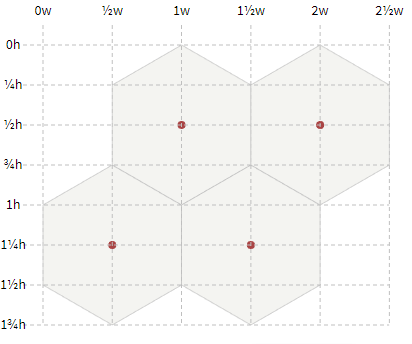
\includegraphics[scale=0.5]{kepek/img61.png}
\caption{Felül hegyes}
\label{fig:img61}
\end{figure}

\begin{figure}[h]
\centering
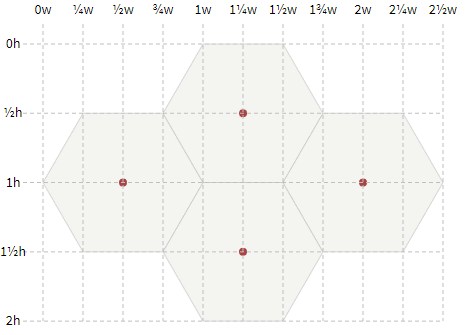
\includegraphics[scale=0.5]{kepek/img62.png}
\caption{Felül lapos}
\label{fig:img62}
\end{figure}

\chapter{Távolság számítás}

\section{Kocka koordináta rendszer}

A kocka koordináta rendszerben, minden hexagon egy kockának felel meg a 3D térben. A szomszédos hexagonok 1 távolságra vannak egymástól a hexagonháló esetén, viszont 2 távolságra vannak egymástól a kocka koordinátarendszerben. Ezáltal téve egyszerűvé a távolságszámítást. A négyzet koordinátarendszer esetén a Manhattan távolság képlet a következő: $abs(dx) + abs(dy)$. A kocka koordinátarendszerben pedig a Manhattan távolság $abs(dx) + abs(dy) + abs(dz)$. Ezekből következik, hogy a hexagon rács esetén a Manhattan távolság képlet a kockarács esetén fentálló távolság fele.
\newline
\newline Pseudo kóddal:
\begin{verbatim}
function cube_distance(a, b):
    return (abs(a.x - b.x) + abs(a.y - b.y) + abs(a.z - b.z)) / 2
\end{verbatim}    

$$
d_{\text{cube}}(a, b) =
\dfrac{|a_x - b_x| + |a_y - b_y| + |a_z - b_z|}{2}
$$

\noindent Egy ezzel egyenértékű megközelítés az is, ha megfigyeljük azt, hogy a három koordináta közül az egyiknek mindenképpen a a másik kettő összegének kell, hogy legyen, ekkor az az egy lesz a távolság. 
\newline
\newline Pseudo kóddal:
\begin{verbatim}
function cube_distance(a, b):
    return max(abs(a.x - b.x), abs(a.y - b.y), abs(a.z - b.z))
\end{verbatim}

$$
d_{\text{cube}}(a, b) =
\max(
|a_x - b_x|, |a_y - b_y|, |a_z - b_z|
)
$$

\noindent Az, hogy melyik algoritmust váltjuk az szituáció és egyén függő, de az eredmény ugyanaz.

\section{Tengelyes koordináta rendszer}

A tengelyes koordináta rendszerben a számításokhoz szükséges három koordinátából kettőt ismerünk, ezért konvertálnunk kell majd a kocka koordináta rendszerre.
\newline
\newline Pseudo kóddal:
\begin{verbatim}
function hex_distance(a, b):
    var ac = axial_to_cube(a)
    var bc = axial_to_cube(b)
    return cube_distance(ac, bc)
\end{verbatim}    

\noindent Egy másik módszer arra az esetre, ha egy függvényben szeretnénk megoldani:
\begin{verbatim} 
function hex_distance(a, b):
    return (abs(a.q - b.q) 
          + abs(a.q + a.r - b.q - b.r)
          + abs(a.r - b.r)) / 2
\end{verbatim}          

\noindent Mivel a tengelyes koordináta rendszerben is a távolságokat kockarács esetén alkalmazható Manhattan távolság számító algoritmussal számítjuk ki, ezért valamilyen módon arra kell visszavezetni.

\section{Eltolásos koordináta rendszer}

Az eltolásos koordináta rendszer esetén is azt a megoldást fogjuk használni amit a tengelyes koordináta rendszer esetén is alkalmaztunk. Átalakítjuk a koordinátákat a kocka koordináta rendszerre.
\newline
\newline Pseudo kód:
\begin{verbatim} 
function offset_distance(a, b):
    var ac = offset_to_cube(a)
    var bc = offset_to_cube(b)
    return cube_distance(ac, bc)
\end{verbatim}  

\chapter{Útkereső algoritmus}

A hexagonok és a négyzetek esetén az útkeresés csak egy ponton különbözik (szomszédok száma) ezért az egyszerűség kedvéért csak a négyzethálónál mutatom be.

\section{Algoritmusok}

A kereső algoritmusokat két pont közötti út megtalálására alkalmazzuk. 
A kereső algoritmusoknak több fajtája van, ezek különbözőképpen közelítik meg a problémát. 
\newline
\newline Az egyik csoport minden esetben talál egy megoldást ami nem feltétlenül a legrövidebb út viszont egy elfogadható közelítése annak (\textit{A algoritmusok}). Ezek az algoritmusok széleskörűen alkalmazhatóak ellentétben a másik csoporttal, mivel azok csak speciális esetekben használhatóak, mivel ezekhez további információk szükségesek a gráfról, amik nem minden esetben állnak rendelkezésünkre.
\newline A másik csoport ami minden esetben az optimális útvonalat találja meg, ha az létezik (\textit{A* algoritmus}).
\newline
\newline Az általános algoritmusok úgy keresik a megoldást, hogy a kezdő ponttól kiindulva végignézik a szomszédos csomópontokat és ezt ismétlik mindaddig amíg meg nem találják a végpontot. Az általános algoritmusok mint például a \textit{széltében először keresés} algoritmus is megtalálja az útvonalat ha megadjuk az ehhez szükséges időt, viszont olyan megoldások amik ''ismerik'' a gráfot általánosságban hamarabb elérik a célt. Gondoljuk csak végig mennyivel egyszerűbb megtalálni egy tárgyat ha tudjuk milyen irányban keressük ellentétben azzal, hogyha minden irányban kellene keresnünk azt.
\newline
\newline Két problémát kell megoldanunk az útkereséssel kapcsolatban 
\begin{itemize}
\item első az útvonal megtalálása két pont között, 
\item a második az, hogy a legrövidebb utat találjuk meg. 
\end{itemize}

\noindent Olyan alapvető algoritmusok mint a \textit{széltében először keresés} vagy a \textit{mélységben először keresés} nagyon egyszerűen megoldják az első problémánkat azáltal, hogy az összes lehetséges útvonalat bejárják. Ezek az algoritmusok $\mathcal{O}(|V| + |E|)$ (lineáris) futásidejűek, ahol $V$ a csúcsok száma és $E$ az élek száma.
\newline
\newline A legrövidebb út megtalálása már ennél jóval komplexebb probléma. 
\newline
\newline Edsger Dijkstra találta meg erre a problémára a megoldást 1956-ban. Az algoritmusából manapság már több változat is létezik. Dijkstra eredeti algoritmusa megtalálta a legrövidebb utat két csúcs között egy súlyozott gráfon, de manapság a leggyakoribb változata úgy változtatja meg az algoritmust, hogy egy megadott csúcsponthoz viszonyítva kiszámítja az összes többi csúcsponthoz vezető legrövidebb utat, ezáltal előállítva a legrövidebb út fát. Ennek a futásideje $\mathcal{O}(|E| + |V| log|V|)$. 
\newline
\newline A \textit{Bellman-Ford} algoritmus ugyanazt a problémát oldja meg mint a \textit{Dijkstra} algoritmus, viszont ez egy sokoldalúbb algoritmus, mivel az élek értéke negatív értéket is felvehet. Mindössze azt kell kizárni, hogy a gráf negatív összköltségű kört tartalmazzon. Negatív költségű él például úgy keletkezhet, hogy nagyobb bevételhez jutunk azon a szakaszon mint amennyi ráfordítással jár. A legrosszabb esetű futásideje $\mathcal{O}(|V||E|)$ (négyzetes idő), de bizonyos esetekben akár $\mathcal{O}(|V|)$ is lehet, ami azt jelenti, hogy legrosszabb esetben lassabb mint a \textit{Dijkstra}-féle algoritmus de akár gyorsabb is lehet. 
\newline
\newline Azonban nem szükséges az összes lehetséges útvonalat bejárni ahhoz, hogy megtaláljuk az optimális útvonalat. Olyan algoritmusok mint a \textit{Dijkstra} vagy az \textit{A*} stratégiája az, hogy heurisztikák segítségével eliminálja az olyan útvonalakat amik nem lehetségesek vagy nem vezetnek a megoldás felé. Ezáltal lehetővé téve, hogy elérjék az $\mathcal{O}(|E| log(|V|))$ futásidőt. 
\newline
\newline A fent említett algoritmusok a legjobb általános algoritmusok közé tartoznak amikkel előfeldolgozás nélkül is kilehet értékelni egy gráfot. Gyakorlatban elérhető még ezeknél is jobb idő komplexitású algoritmus, ha előfeldolgozzuk a gráfot.
\newline
\newline A leggyakrabban alkalmazott algoritmusok ismertetése:

\subsection{Széltében először keresés algoritmus (breadth-first search)}
A \textit{széltében először keresés} egy egyszerűnek számító keresési algoritmus. A térképen minden egyes irányban egységes mértékben keres. Ez egy teljes keresés, ezáltal minden esetben a legrövidebb utat fogja megtalálni a célhoz. A keresés a gyökér csomóponttól indul és úgy folytatódik, hogy az összes csomópontot ami a gyökér csomópontból elérhető kiértékeli. Ezután ezekből a csomópontokból elérhető csomópontokat értékeli ki az algoritmus. Ez az algoritmus mindig egy adott mélységen lévő csomópontokat értékeli ki egyszerre és ezután halad tovább a következő szintre. Könnyen belátható, hogy az algoritmus a FIFO (first-in-first-out) elv alapján működik. Tehát azokat az elemeket értékeli ki először egy adott listáról amik először felkerültek a listára. Ezáltal belátható, hogy ez az algoritmus a legmagasabb szinten található cél csomópontot fogja megtalálni először. 

\begin{figure}[h!]
\centering
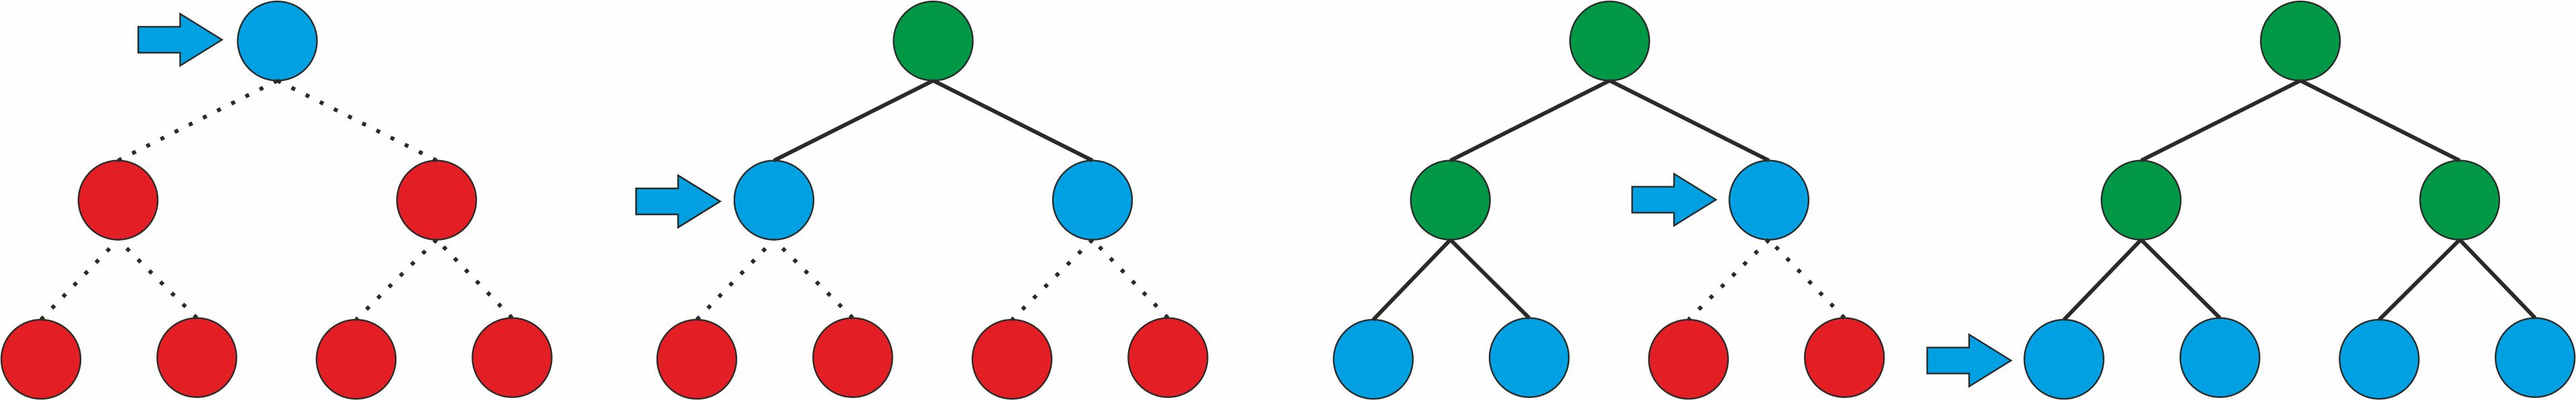
\includegraphics[scale=0.4]{kepek/breadth-first_search.jpg}
\caption{Széltében először keresés algoritmus lépései}
\label{fig:breadth-first_search}
\end{figure}

\noindent Mindazonáltal mivel ez egy teljes keresés az egész gráf kiértékelésre kerül, mivel nem feltétlenül a legmagasabban található cél csomóponthoz vezető úton jutunk el a leggyorsabban a célhoz, abban az esetben ha az éleknek különbözik a súlya. Ezért érdemes olyan esetekben használni amikor a gráf éleinek nincs súlya vagy egységes súlya van, mert abban az esetben elégséges lehet a legmagasabban található cél csomópontig eljutni.  Érdemes továbbá tisztázni, hogy ha a térképen egy darab célpontunk van az a gráfban több célcsomópontként is megjelenhet, mivel a gráf különböző útvonalai a különböző útvonalakat jelölik ugyanazon célhoz, de egyszerre akár több célunk is lehet a térképen.
\newline
\newline A széltében először keresés algoritmus legnagyobb hátránya a tárigénye. Vegyünk például egy hipotetikus állapotteret, ahol minden kifejtéskor $x$ darab új csomópontot kapunk állapotunk van. Tehát a gyökér kifejtésekor $x$ darab elemünk lesz. Második szinten $x^2$. Tegyük fel, hogy a cél csomópontunk n mélységben található, ekkor legrosszabb esetben $x^n - x$ csomópontot kell kiértékelnünk, mivel az utolsó mélységet már nem szükséges kiértékelnünk. 
\newline
\newline A széltében először keresés algoritmus egy nem informált keresés mivel a cél csomópontról nem rendelkezik információval. A továbbiakban csak informált keresésekről esik majd szó.

\subsection{Dijkstra algoritmus}

\noindent Gyakori példa a gráf alapú útkereső algoritmusra a \textit{Dijkstra} algoritmus. A széltében először keresés módszerrel ellentétben nem egységesen fedezi fel az utakat, hanem a kisebb útköltségűeket priorizálja. Ennek az algoritmusnak az elején szükségünk lesz egy kezdő csomópontra és egy listára a “Nyitott” csomópontoknak, ide kerülnek azok a csomópontok amiket még ki kell értékelnünk. Minden iterációban az a csomópont kerül kiértékelésre amelyiknek a legkisebb az útköltsége a kezdő csomóponttól mérve. Az útköltség függhet attól, hogy milyen területen haladunk (magassági viszonyok változásától, a talaj anyagától, időjárási viszonyoktól, egyéb környezeti viszonyoktól, ha az úton ellenség van akkor is megnövelhetjük az út költségét). Az algoritmus alapvetően súlyozott élek esetén működik, de használható súlyozatlan élek esetén is, ekkor a súlyozatlan élek értékét válasszuk 1-nek. Akkor kerül egy csomópont “lezárásra”, hogyha már az összes szomszédja hozzá lett adva a nyitott csomópontok listájához vagy már lezárásra került. Ez a folyamat addig ismétlődik amíg az algoritmus megtalálja az első útvonalat a célhoz (ami lehet akár az összes csomópont is). Mivel mindig a legkisebb útköltségre lévő út fog kiértékelődni, ezért amit először megtalál, az lesz a legrövidebb út. Tehát változatos útköltségek esetén érdemesebb a \textit{Dijkstra} algoritmust használni a széltében először keresés módszer helyett.

\subsection{A* algoritmus}

\noindent Az \textit{A*} algoritmus a \textit{Dijkstra} algoritmus tovább gondolása, amit gyorsasága és a pontossága miatt előszeretettel alkalmaznak játékok készítésekor, olyan esetekben, amikor csak egy konkrét végponthoz kell eljutni. A két algoritmus közötti fő különbség abban rejlik, hogy melyik csomópontot választja ki az algoritmus kiértékelésre a nyitott csomópontok közül. Ahhoz, hogy megértsük az \textit{A*} kiválasztási módszerét először meg kell ismernünk 3 fogalmat.

\begin{itemize}
\item \textit{G költség}: Az adott csomóponthoz vezető út költsége a kezdő csomóponthoz képest.
\item \textit{H költség (heurisztikus költség)}: A becsült távolság a célhoz képest.
\item \textit{F költség}: $F = G + H$. Ez az érték alapján kerül kiválasztásra a kiértékelendő csomópont.
\end{itemize}

\noindent A \textit{Dijkstra} algoritmussal ellentétben nem az útköltségek alapján priorizál hanem a célponttól lévő távolság alapján.
\newline
\newline A \textit{G költség} tulajdonképpen a \textit{Dijkstra} algoritmus használata és ezt egészíti ki az \textit{A*} algoritmus egy heurisztikus költséggel, ami azért szükséges, hogy kizárjuk a hosszabb útvonalakat. Heurisztikaként leggyakrabban a Manhattan-formulát szokták használni. Ha a heurisztikus költséget 0-ra ''állítjuk be'', akkor az algoritmus megegyezik a \textit{Dijkstra} algoritmussal.
\newline
\newline Az útkereső algoritmus készítéséhez szükséges ismernünk azt, hogy a térkép egy mezőjéről hogyan érhetőek el a szomszédos mezők és szükséges ismernünk a távolság számító algoritmusokat is. Mivel a távolság számító algoritmusokat már ismertettem korábban ezért most nézzük meg a szomszédokat.

\section{Szomszédok}

Ahhoz, hogy útkereső algoritmust tudjunk készíteni ismernünk kell, hogy a különböző alakzatok és koordináta-rendszerek esetén milyen algoritmussal érhetjük el az adott alakzat szomszédait. 
\newline
\newline Az algoritmusokat ebben a formában fogom megadni: $A \rightarrow B1, B2, B3 …$
(Az $''A''$ és $''B''$ pontokat $''u''$, $''v''$ koordináták segítségével fogom megadni.)

\subsection{Négyzet}
A négyzet esetén egyszerű dolgunk van, mert csak egyfajta koordináta-rendszerünk van.

$$
(u,v) \rightarrow (u,v+1) (u+1,v) (u,v-1), (u-1,v)
$$

\subsection{Hexagon}

Hexagon esetén több fajta koordináta-rendszerünk is lehet.

\subsubsection{Kocka koordináta-rendszer (Cube coordinates)}

\noindent Ahhoz, hogy elmozduljunk eggyel meg kell változtatnunk egyet a három kocka koordináta közül $+1$-el és egy másikat $-1$-el (a változtatások összege $0$ kell, hogy legyen). Három koordinátát lehet megváltoztatni $+1$-el, a másik két lehetséges koordináta közül az egyiket kell csökkenteni $-1$-el. Ez hat lehetséges változatot eredményez. Mindegyik megfeleltethető a hexagon egyik irányának. A lehető legegyszerűbb és leggyorsabb megoldás az, ha az összes lehetséges permutációt előre kikalkuláljuk és beleírjuk egy táblázatba ( Cube($dx, dy, dz$)).
\newline
\newline Algoritmus: 
\begin{verbatim}
var cube_directions = [
   Cube(+1, -1,  0), Cube(+1,  0, -1), Cube( 0, +1, -1),
   Cube(-1, +1,  0), Cube(-1,  0, +1), Cube( 0, -1, +1)
]

function cube_direction(direction):
    return cube_directions[direction]

function cube_neighbor(cube, direction):
    return cube_add(cube, cube_direction(direction))
\end{verbatim}

\subsubsection{Tengely koordináta-rendszer (Axial coordinates)}

\noindent A kocka koordináta-rendszer veszük alapul. Mégpedig úgy, hogy a Cube($ dx, dy, dz$) koordinátákat átalakítjuk Axial($ dx, dz$) -re.
\newline
\newline Algoritmus:
\begin{verbatim}
var axial_directions = [
   Hex(+1,  0), Hex(+1, -1), Hex( 0, -1),
   Hex(-1,  0), Hex(-1, +1), Hex( 0, +1)
]

function hex_direction(direction):
    return axial_directions[direction]

function hex_neighbor(hex, direction):
    var dir = hex_direction(direction)
    return Hex(hex.q + dir.q, hex.r + dir.r)
\end{verbatim}

\subsubsection{Eltolásos koordináta-rendszer (Offset coordinates)}

\noindent Eltolásos koordináta-rendszer esetén a lépések változnak annak a függvényében, hogy hol állunk a hálóban. Ha mi egy eltolt oszlopban/sorban állunk akkor a szabály eltér attól mintha egy nem eltolt oszlopban/sorban állnánk.
\newline
\newline Ahogy a korábbi esetekben úgy most is kell készítenünk egy táblázatot amiben azt tároljuk majd, hogy a különböző tengelyeken mennyit kell hozzáadni, hogy elérjük a szomszédokat. De ebben az esetben most két tömbre lesz szükségünk, az egyik a páros sor/oszlop a másik pedig a páratlan sor/oszlop esetére.
\newline
\newline A táblázat különbözik mind a négy eltolásos módszernél.
\newline
\newline Páratlan sor: 
\begin{verbatim}
var oddr_directions = [
   [ Hex(+1,  0), Hex( 0, -1), Hex(-1, -1),
     Hex(-1,  0), Hex(-1, +1), Hex( 0, +1) ],
   [ Hex(+1,  0), Hex(+1, -1), Hex( 0, -1),
     Hex(-1,  0), Hex( 0, +1), Hex(+1, +1) ]
]

function oddr_offset_neighbor(hex, direction):
    var parity = hex.row & 1
    var dir = oddr_directions[parity][direction]
    return Hex(hex.col + dir.col, hex.row + dir.row)
\end{verbatim}
Páros sor: 
\begin{verbatim}
var evenr_directions = [
   [ Hex(+1,  0), Hex(+1, -1), Hex( 0, -1),
     Hex(-1,  0), Hex( 0, +1), Hex(+1, +1) ],
   [ Hex(+1,  0), Hex( 0, -1), Hex(-1, -1),
     Hex(-1,  0), Hex(-1, +1), Hex( 0, +1) ]
]

function evenr_offset_neighbor(hex, direction):
    var parity = hex.row & 1
    var dir = evenr_directions[parity][direction]
    return Hex(hex.col + dir.col, hex.row + dir.row)
\end{verbatim}
Páratlan oszlop: 
\begin{verbatim}
var oddq_directions = [
   [ Hex(+1,  0), Hex(+1, -1), Hex( 0, -1),
     Hex(-1, -1), Hex(-1,  0), Hex( 0, +1) ],
   [ Hex(+1, +1), Hex(+1,  0), Hex( 0, -1),
     Hex(-1,  0), Hex(-1, +1), Hex( 0, +1) ]
]

function oddq_offset_neighbor(hex, direction):
    var parity = hex.col & 1
    var dir = oddq_directions[parity][direction]
    return Hex(hex.col + dir.col, hex.row + dir.row)
\end{verbatim}
Páros oszlop: 
\begin{verbatim}
var evenq_directions = [
   [ Hex(+1, +1), Hex(+1,  0), Hex( 0, -1),
     Hex(-1,  0), Hex(-1, +1), Hex( 0, +1) ],
   [ Hex(+1,  0), Hex(+1, -1), Hex( 0, -1),
     Hex(-1, -1), Hex(-1,  0), Hex( 0, +1) ]
]

function evenq_offset_neighbor(hex, direction):
    var parity = hex.col & 1
    var dir = evenq_directions[parity][direction]
    return Hex(hex.col + dir.col, hex.row + dir.row)
\end{verbatim}

\subsubsection{Átlós szomszédok}

\noindent Az “átlós” szomszédok a kocka koordináták esetén úgy működik, hogy a lehetséges három koordináta közül az egyiket $ \pm 2$ -vel, míg a másik kettőt $\mp 1$ -el módosítjuk, hogy a három koordináta összege mindig $0$ legyen.

\begin{figure}[h!]
\centering
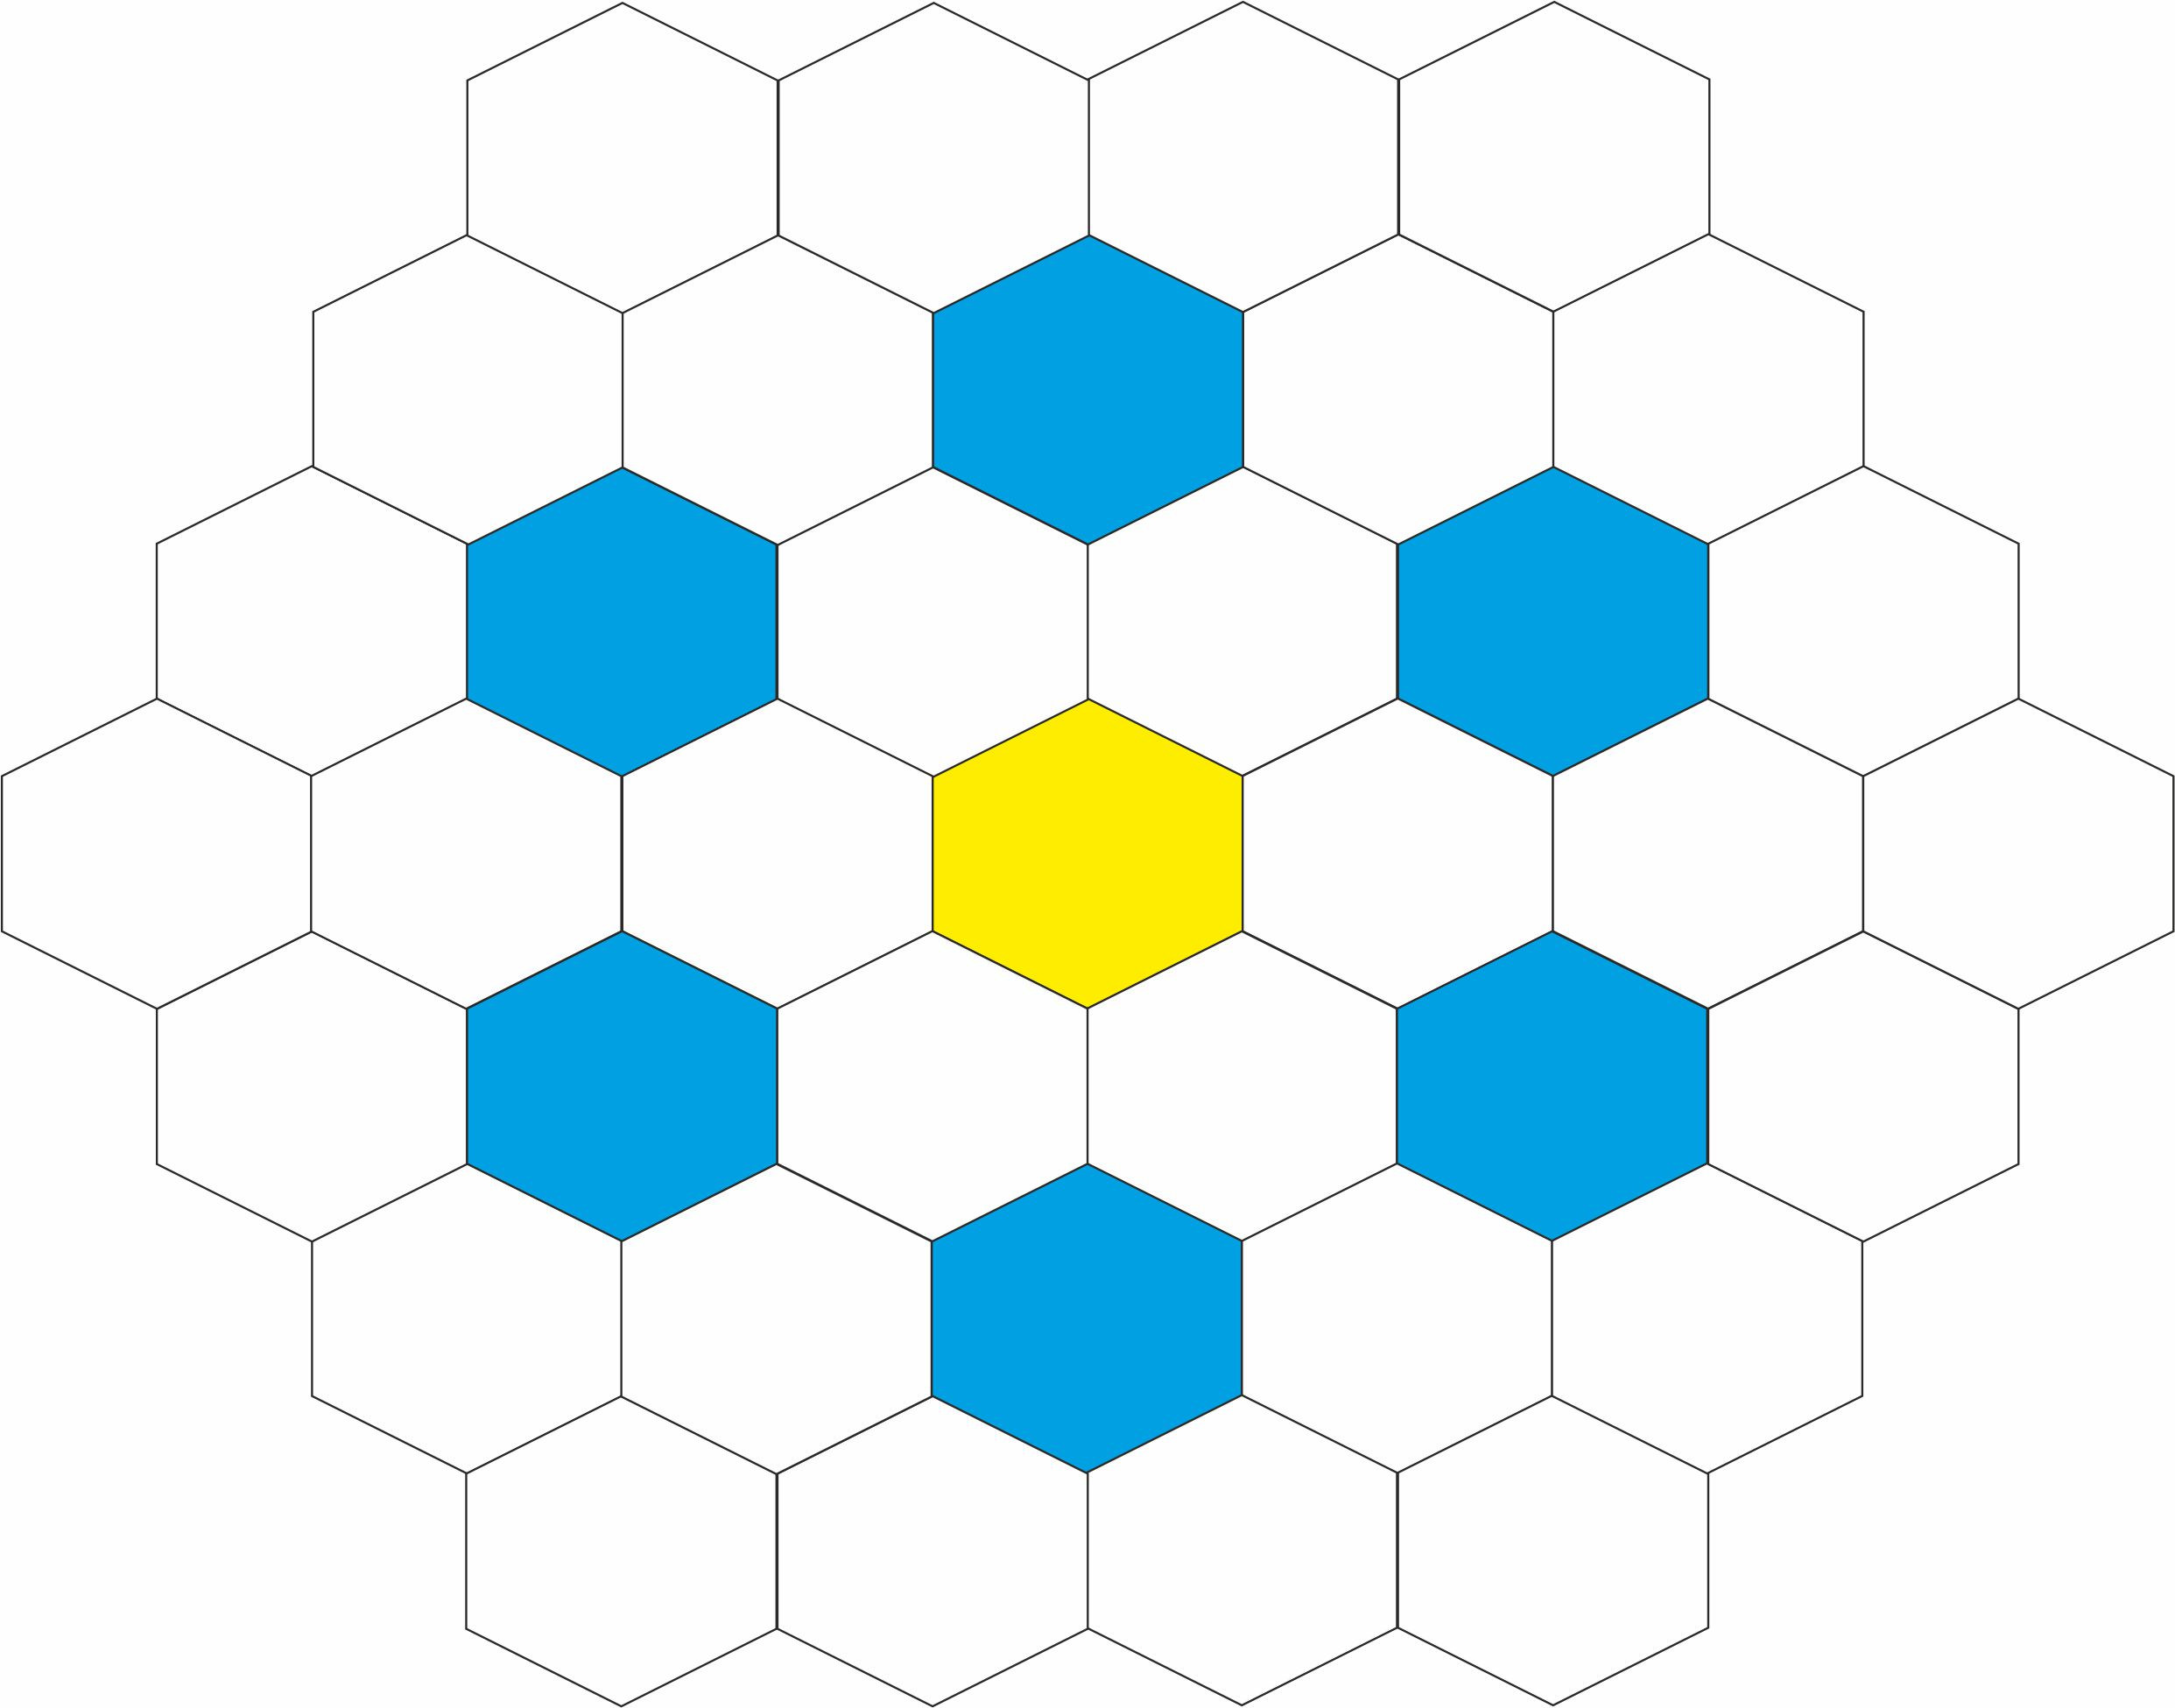
\includegraphics[scale=0.3]{kepek/Diagonals.jpg}
\caption{"Átlós" szomszédok hexagon háló esetén}
\label{fig:Diagonals}
\end{figure}

\noindent Algoritmus:
\begin{verbatim}
var cube_diagonals = [
   Cube(+2, -1, -1), Cube(+1, +1, -2), Cube(-1, +2, -1), 
   Cube(-2, +1, +1), Cube(-1, -1, +2), Cube(+1, -2, +1)
]

function cube_diagonal_neighbor(cube, direction):
    return cube_add(cube, cube_diagonals[direction])
\end{verbatim}

\noindent Tengelyes koordináta-rendszer használata esetén is lehetséges az algoritmus használata.
\Chapter{Térkép generálása}

\section{Metrikák}

A hexagonok és a négyzetek esetén az útkeresés csak egy ponton különbözik (szomszédok száma) ezért az egyszerûség kedvért csak a négyzethálónál mutatom be

hexagon
offset coord
pointy top

Bemenetként a térkép fõ jellemzõit, a generált térképpel szembeni elvárásokat kapja paraméterezésként.

A térkép egy több lépcsõs folyamat végén fog elkészülni. 
Az elsõ fázisban a nagyobb területi egységek (szigetek, folyók, ...) körvonalazódása történik. 
A második lépésben a térkép alapegységeinek (tile) a konkretizálása történik meg, azaz leképzõdik egy hexagon háló. 
Harmadik lépésként minden egyes tile-hoz hozzárendeli az algoritmus a megfelelõ textúrát a területi egységek alapján. 
A negyedik fázisban városokat, településeket, falakat hoz létre a program. 
Ötödik lépésként a növényzetet (fák, bokrok) generálja majd le. 
A hatodik lépésben a dekorálás jön, ahol az évszakoknak és a különbözõ természeti hatásoknak megfelelõen módosulhat a textúra.

Elsõ lépésként szükségünk lesz egy csempére (tile), ami az alapelem lesz a térképen. Erre a célra én egy 3D-s hexagon modellt használtam különbözõ textúrákkal.

Ezen kívül szükség van a generálni kívánt térkép méreteire (szélesség, magasság).


\chapter{Összefoglalás}

A szakdolgozatom célja egy olyan procedurális generálási mód megvalósítása volt, ami változatos térképet generál izometrikus grafikájú játékokhoz. Az elméleti ismeretek bemutatása után az általam preferált technikák kiválasztásának indoklása és az implementálásukhoz szükséges részletek kifejtése történt meg. Végezetül a program implementációjának bemutatása következett. A szakdolgozatom során igyekeztem ábrákkal segíteni az általam kevésbé egyértelműnek tűnő részeket. 

\bigskip

\noindent A szakdolgozatom készítése során sikerült létrehoznom egy olyan algoritmust amely a megadott bermeneti értkek alapján állít elő "véletlenszerű" térképet. A programomnak vannak még hiányosságai, amely további fejlesztést igényel.

\bigskip

\noindent Az alkalmazás további fejlesztésére különféle lehetőségek vannak. Az alábbiakban felvetés szintjén szerepel ezek közül néhány.
\begin{itemize}
\item A program optimalizálása különböző területeken (kód, teljesítmény).
\item További objektumok (épületek/növények/utak/hidak/állatok) hozzáadása, hogy sokszínűbb térképet kapjunk.
\item Lehetőség arra, hogy lementsük és betöltsük a térképet.
\item Napszakok és további időjárásbeli (eső,hó,köd) tényezők létrehozása, ezáltal változatosabb környzet kialakítása. 
\end{itemize}


\begin{thebibliography}{x}
\addcontentsline{toc}{chapter}{\bibname}

\bibitem{Daggerfall} https://en.wikipedia.org/wiki/The\_Elder\_Scrolls\_II:\_Daggerfall (2017.11.22)
\bibitem{Civ1} https://en.wikipedia.org/wiki/Civilization\_(series)
\bibitem{Spore} https://en.wikipedia.org/wiki/Development\_of\_Spore\#Procedural\_generationhttps://en.wikipedia.org/wiki/Development\_of\_Spore (2017.11.22)
\bibitem{RTS_Camera} https://www.assetstore.unity3d.com/en/\#!/content/43321 (2017.11.22)










\bibitem{algoritmusok} Thomas H. Cormen, Charles E. Leiserson, Ronald L. Rivest. (2001). Algoritmusok. Műszaki Könyvkiadó.
\bibitem{HexagonalGrids} http://www.redblobgames.com/grids/hexagons/ (2017.11.22)
\bibitem{A*} http://www.redblobgames.com/pathfinding/a-star/introduction.html (2017.11.22)
\bibitem{Grids} http://www-cs-students.stanford.edu/$\tilde{}$amitp/game-programming/grids/ (2017.11.22)
\bibitem{HexMap} http://catlikecoding.com/unity/tutorials/hex-map/part-1/ (2017.11.22)
\bibitem{HexagonalGrids} http://keekerdc.com/2011/03/hexagon-grids-coordinate-systems-and-distance-calculations/ (2017.11.22)
\bibitem{Dijkstra} https://en.wikipedia.org/wiki/Dijkstra\%27s\_algorithm (2017.11.22)







\bibitem{Pathfinding} https://en.wikipedia.org/wiki/Pathfinding (2017.11.22)
\bibitem{A*} https://en.wikipedia.org/wiki/A*\_search\_algorithm (2017.11.22)

\bibitem{Breadth-first_search} https://en.wikipedia.org/wiki/Breadth-first\_search (2017.11.22)

\bibitem{Procedural_generation} https://en.wikipedia.org/wiki/Procedural\_generation (2017.11.22)




\bibitem{CIV-V} http://www.firaxis.com/?/blog/single/procedural-terrain-generation-in-sid-meiers-civilization-v (2017.11.22)
\bibitem{Dispatcher} https://github.com/nickgravelyn/UnityToolbag/tree/master/Dispatcher (2017.11.22)
\bibitem{Unity} https://www.assetstore.unity3d.com (2017.11.22)

\bibitem{LowPolyPack ?hegyek?} https://www.assetstore.unity3d.com/en/\#!/content/58821 (2017.11.22)


\end{thebibliography}


% %Az összefoglaló fejezet
\chapter*{Adathordozó használati útmutató}
\addcontentsline{toc}{chapter}{Adathordozó használati útmutató}

%Ebben a fejezetben kell megadnunk, hogy a szakdolgozathoz mellékelt adathordozót (pl. CD) hogyan lehet elérni, milyen strukturát követ. Minimum 1 maximum 4 oldal a terjedelem. Lehet benne több alszakasz is. A fejezet címe nem módosítható, hasonlóan a következõ részhez (Irodalomjegyzék).

% TODO: Mindenhova egész mondatok kellenének majd.

\noindent A szakdolgozatomhoz mellékelt adathordozó eszközön található jegyzékek és fájlok az alábbiak.

\bigskip

\noindent \texttt{$\backslash$FelhasznaloiDokumentacio.pdf}

\medskip

Felhasználói dokumentáció

\bigskip

\noindent \texttt{$\backslash$FuttathatoValtozat}

\medskip

Futtatható változatot tartalmazó jegyzék az összes szükséges bináris állománnyal.

\bigskip

\noindent \texttt{$\backslash$FuttathatoValtozat$\backslash$Szakdolgozat.exe}

\medskip

A futtatható állomány.

\bigskip

\noindent \texttt{$\backslash$KodForrasszovege}

\medskip

Kód forrásszövegét tartalmazó jegyzék

\bigskip

\noindent \texttt{$\backslash$SzakdolgozatTeljesSzovege.pdf}

\medskip

Szakdolgozat teljes szövege

\bigskip

\noindent \texttt{$\backslash$Kepek}

\medskip

Az alkalmazásról képeket tároló jegyzék


\end{document}

